%% 
%% Copyright 2019-2020 Elsevier Ltd
%% 
%% This file is part of the 'CAS Bundle'.
%% --------------------------------------
%% 
%% It may be distributed under the conditions of the LaTeX Project Public
%% License, either version 1.2 of this license or (at your option) any
%% later version.  The latest version of this license is in
%%    http://www.latex-project.org/lppl.txt
%% and version 1.2 or later is part of all distributions of LaTeX
%% version 1999/12/01 or later.
%% 
%% The list of all files belonging to the 'CAS Bundle' is
%% given in the file `manifest.txt'.
%% 
%% Template article for cas-dc documentclass for 
%% double column output.

% \documentclass[a4paper,fleqn]{cas-dc}
\documentclass[a4paper,fleqn]{DC_ArtStyle}
% \documentclass[]{interact}

% \usepackage[authoryear,longnamesfirst]{natbib}
% \usepackage[authoryear]{natbib}
\usepackage[numbers]{natbib}
\usepackage{lipsum}
\usepackage{xcolor}
\usepackage{caption}
\usepackage{subcaption}
\usepackage{siunitx}
\usepackage{array}
\usepackage{multirow}
\usepackage{amsmath}
\usepackage{amssymb}
\usepackage{rotating}
\usepackage{float}
\usepackage{multicol}
\usepackage{pdfpages}
\usepackage[normalem]{ulem}
\usepackage[justification=centering]{caption}
\usepackage{cuted}


\newcommand{\abbreviations}[1]{%
	\nonumnote{\textit{Abbreviations:\enspace}#1}}

\setlength{\parindent}{0pt}

\begin{document}
	\let\WriteBookmarks\relax
	\def\floatpagepagefraction{1}
	\def\textpagefraction{.001}
	\shorttitle{Fabric-Elasticity Property Relationships of the Human Cortical Femur}
	\shortauthors{Simon et~al.}
	
	\title[mode = title]{Fabric-Elasticity Property Relationships of the Human Cortical Femur}
	
	% Autors
	\author{Mathieu Simon}
	\ead{mathieu.simon@artorg.unibe.ch}

    \author{Gabriela Gerber}
    
    \author{Simone Poncioni}

	\author{Yvan Gugler}

	\author{Kurt Lippuner}

	\author{Philippe Zysset}
	\ead{philippe.zysset@artorg.unibe.ch}

	
	% Adresses
	\address{ARTORG Centre for Biomedical Engineering Research, University of Bern, Bern, Switzerland}
	
	% Abbreviations
	\abbreviations{%
		ROI, region of interest;
		\textmu CT, micro-computed tomography;
		}
	
	% Footnotes
	
	%
	%
	%
	% ABSTRACT
	%
	%
	%
	
	\begin{abstract}
		Lorem ipsum dolor sit amet, consectetuer adipiscing elit.
		Utpurus elit, vestibulum ut, placerat ac, adipiscing vitae, felis.
		Curabitur dictum gravida mauris.
		Nam arcu libero, nonummy eget, consectetuer id, vulputate a, magna.
		Donec vehicula augue eu neque.
		Pellentesque habitant morbi tristique senectus et netus et malesuada fames ac turpis egestas.
		Mauris ut leo. Cras viverra metus rhoncus sem.
		\\[0.5em]
		Nulla et ectus vestibulum urna fringilla ultrices.
		Phasellus eu tellus	sit amet tortor gravida placerat.
		Integer sapien est, iaculis	in, pretium quis, viverra ac, nunc.
		Praesent eget sem vel leo ultrices bibendum.
		Aenean faucibus. Morbi dolor nulla,	malesuada eu, pulvinar at, mollis ac, nulla.
		Curabitur auctor semper nulla.
		Donec varius orci eget risus.
		Duis nibh mi, congue eu, accumsan eleifend, sagittis quis, diam.
		Duis eget orci sit amet orci dignissim rutrum.
		\\[0.5em]
		Nam dui ligula, fringilla a, euismod sodales, sollicitudin vel, wisi.
		Morbi auctor lorem non justo.
		Nam lacus libero, pretium at, lobortis vitae, ultricies et, tellus.
		Donec aliquet, tortor sed accumsan bibendum, erat ligula aliquet magna, vitae ornare odio metus a mi.
		Morbi ac orci et nisl hendrerit mollis.
		Suspendisse ut massa.
		Cras nec ante.
		Pellentesque a nulla.
		Cum sociis natoque penatibus et magnis dis parturient montes, nascetur ridiculus mus.
		Aliquam tincidunt urna.
		Nulla ullamcorper vestibulum turpis.
		Pellentesque cursus luctus mauris.
    \end{abstract}
	
	\begin{keywords}
		Bone \sep%
		Fabric \sep%
		Elasticity \sep%
	\end{keywords}
	

	\begin{NoHyper}
		\maketitle
	\end{NoHyper}
	
	%
	%
	%
	% INTRO
	%
	%
	%
	
	\section{Introduction}
	Bone is a hierarchically structured natural material mainly composed of hydroxyapatite (HA), collagen type I, and water \cite{Fratzl2007NaturesHM}.
	At the nanoscale, collagen molecules self-assemble to form fibrils staggered into their longitudinal direction width a gap of about 67 nm between adjacent molecules.
	In this gap, HA aggregate to form cristals leading to mineralisation of collagen fibrils.
	These mineralised collagen fibrils are arranged together into lamellae and this so-called lamellar bone is the building block of the two main bone structures observed at the macroscale: cortical and trabecular bone.\\

	In cortical bone, lamellae are arranged concentrically around Haversian canals to form osteons.
	The Haversian canal contains nerves, blood, and lymphatic vessels and measure about 70 \textmu m in diameter while the complete osteon is about 100-200 \textmu m in diameter.
	At their external surface, osteons are bounded by a thin layer called the cement line, separating it from the older interstitial bone tissue.
	Altogether, they form the cortical bone tissue, being the outer shell of bones, with a porosity varying between 5 and 15\%.
	Towards the inside and the epiphyses of bones, porosity of the bone tissue increases leading to trabecular bone structure.
	In trabecular bone, bone lamellae are concentrically arranged to form trabeculae and the porosity, ranging from 20 to 90\%, is represented by the inter-trabecular space.\\

	With ageing, a metabolic imbalance leads to a progressive loss of bone mass.
	This decrease of bone mass weakens the skeleton, increasing fracture risk, and ultimately leading to osteoporosis.
	It is estimated that 1/5 men and 1/3 women over 65 years old will experience a fragility fracture induced by a load that shouldn't have caused a fracture in normal conditions.
	These fractures lead to pain, increased costs for the society, and an increased morbidity.
	The gold standard for the assessment of osteoporosis is dual-energy X-ray absorptiometry (DXA), typically performed at the lumbar spine or the femoral neck.
	DXA results in an areal bone mineral density (aBMD) value which is then compared to a reference population.
	However, DXA misses of specificity as an important part of fragility fractures happens to people above the osteoporosis threshold.
	Therefore, clinicians are looking for better surrogate to estimate bone strength.\\

	High-resolution peripheral quantitative computed tomography (HR-pQCT) allows acquiring in vivo scans of the bone structure at peripheral sites such as the radius and tibia.
	These scans can serve as a basis for numerical analysis allowing to estimate bone strength.
	One way to perform these simulations is to convert every voxel to finite element and modelize a compression of the scanned section.
	This approach then leads to models containing millions of \textmu m-sized finite elements which require heavy computational effort to solve.
	Another approach consists of using milimeter-sized elements, so-called homogenized finite elements (hFE) and corresponding constitutive models.
	This second approach, while being a less accurate representation of the bone geometry, lead to models considerably lighter to solve.
	Additionally, it was shown that such hFE models are able to provide accurate bone strength assessment.
	However, such models highly depend on the constitutive model used to describe the bone's tissue mechanical behavior.\\

	The mechanical properties of bone tissue are usually assessed using experimental approaches.
	\textcolor{red}{Cite studies showing experimental assessment of bone mechanical properties}.
	However, bone tissue properties can also be assessed via numerical approach.
	\textcolor{red}{Cite studies assessing bone properties using \textmu FE.}
	As mentioned previously, \textmu FE require expensive resources for large models.
	Therefore, hFE becomes an attractive alternative using adapted constitutive relations.
	
	Over the years, many constitutive models have been proposed to describe the mechanical behavior of bone.
	\textcolor{red}{
	Introduce the different models.
	Describe density and fabric.
	Introduce the Yang and Cowin model as well as the Zysset-Curnier model.
	Present investigations performed for trabecular bone}
	However, these relationships are not yet verified for cortical bone.\\

	\textcolor{red}{
	Constitutive model are compared to mechanical experiments and numerical simulations.
	For cortical bone, nanoindentation experiment have shown that bone matrix is transverse isotropic.
	Combined with micro-computed tomography, it is possible to simulate the mechanical behavior of millimeter-size cortical bone samples.
	Experimentally, resonant ultrasound spectroscopy (RUS) measurements allows for estimation of elasticity tensor of cortical bone.
	}\\

	The aim of the present study is to investigate the influence of the bone matrix properties and microstructure on the mechanical properties of human bone.
	The relationships between density, fabric and mechanics are presented from the bone matrix (bone of full density) down to the low density of trabecular bone with a strong focus on the cortical bone.
	Additionally to relationships description, the objective is to provide material constants for bone properties estimation.

	%
	%
	%
	% METHODS
	%
	%
	%
	
	\newpage
	\section{Material and Methods}
	The \textmu CT scans and corresponding mechanical data of cortical bone used in this study were provided by the Sorbonne Université, INSERM, CNRS, Laboratoire d'Imagerie Biomédicale (LIB), F-75006 Paris, France.
	The detailed process of the sample preparation, scanning and measurement is provided in the study of \citeauthor{Cai2019AnisotropicEP}\cite{Cai2019AnisotropicEP}.
	Briefly, rectangular parallelepiped samples of about 3x4x5 mm (radial, circumferential, and axial direction, respectively) were thawed from both lateral and medial part of the left femur from 29 human cadavers.
	The elasticity tensor of these samples was measured using resonant ultrasound spectroscopy (RUS) \cite{Bernard2013AccurateMO}, assuming transverse isotropy.
	After mechanical measurement, the samples were scanned using synchrotron radiation micro-computed tomography (SR-\textmu CT) at the European Synchrotron Radiation Facility (ESRF, Grenoble, France).
	The original voxel size of these scans of 6.5 \textmu m was coarsened by a factor 2, allowing a good compromise between computational efficiency and structural accuracy.
	After coarsening, 16 cubic regions of interest (ROIs) of 1 mm side length were selected uniformly over the sample.
	A typical cortical sample with its porosities and the distribution of the selected ROIs are shown in Figure \ref{FigCortSamples}.

	\begin{figure}[!h]
		\centering
		\begin{subfigure}[t]{.45\linewidth}
			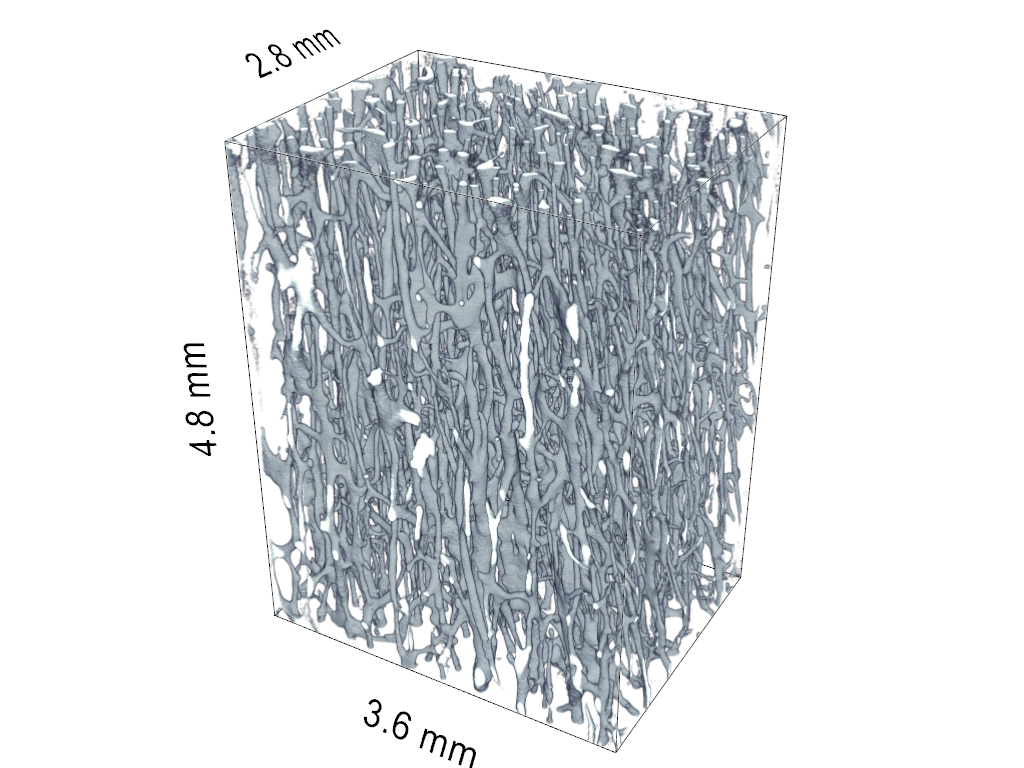
\includegraphics[height=0.8\linewidth]{../Results/Scans/2009_213_L}
			\caption{Typical sample with its porosities}
		\end{subfigure}
		\begin{subfigure}[t]{0.45\linewidth}
			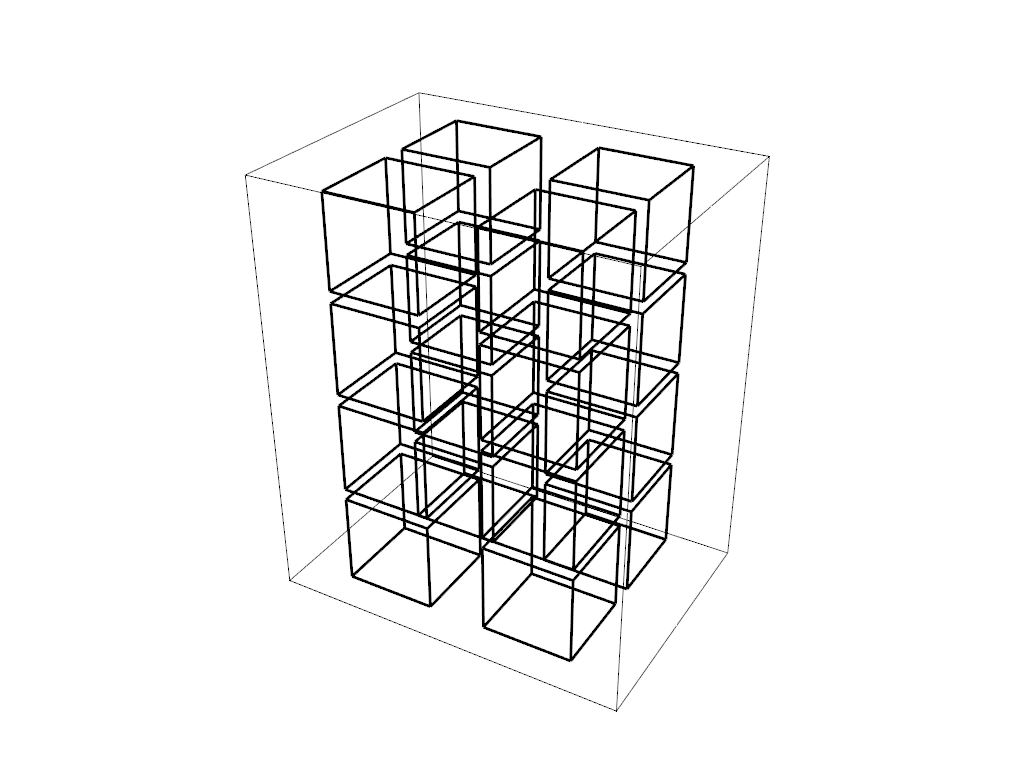
\includegraphics[height=0.8\linewidth, trim=50 50 50 0]{../Results/ROIs/ROIs}
			\caption{ROIs selected for analysis}
		\end{subfigure}
		\label{FigCortSamples}
	\end{figure}

	The CT scans of trabecular bone samples were produced in a previous study \cite{Simon2021FabricelasticityRO} using high-resolution peripheral quantitative computed tomography (HR-pQCT).
	Briefly, HR-pQCT scans were performed on 120 healthy individuals' tibia with a voxel size of about 61 \textmu m.
	Then, 6 cubic ROIs of 5.2 mm side length were randomly selected within the proximal stack of the scan, leading to a total of 720 ROIs.\\

	Both cortical and trabecular bone ROIs underwent numerical homogenisation.
	The homogenisation process was performed using medtool (Dr. Pahr Ingenieurs e.U., Pfaffstätten, Austria) for pre- and postprocessing and ABAQUS (Dassault Syst{\`e}mes Simulia Corp) for numerical simulation.
	The homogenisation scheme consist of simulating 6 loadcases (3 compression and 3 pure shearing) imposing an apparent strain of about 0.001 with kinematic uniform boundary conditions (KUBCs) and computing the resulting apparent stress.
	The bone geometry was generated by segmenting the ROIs using the mean Otsu threshold of each group.
	Then, every voxel segmented as bone tissue was converted to an haxahedral element.
	For trabecular ROIs, an isotropic material was assumed with a Young's modulus of 10 GPa and a Poisson's ratio of 0.3.
	For cortical ROIs, the simulations were performed using 2 different material.
	First, an isotropic material with the same properties as for trabecular ROIs.
	Second, a transversely isotropic material with the plane of symmetry perpendicular to the scan 3\textsuperscript{rd} axis.
	The properties of transversely isotropic material were determined from nanoindentation results of cortical bone presented in the work of \citeauthor{Franzoso2009ElasticAO}\cite{Franzoso2009ElasticAO} and \citeauthor{DallAra2012MicroindentationCD}\cite{DallAra2012MicroindentationCD}, see Table \ref{TableTransProps}.

	\begin{table*}
		\caption{Nanoindentation - cortical bone matrix properties}
		\resizebox{\linewidth}{!}{%
		\begin{tabular}{l|c|c|c|c|c|c|c|c|c}
			Study & E1 & E2 & E3 & Nu12 & Nu13 & Nu23 & Mu12 & M13 & Mu23 \\
			\hline
			Dall'Ara & & & & & & & & & \\
			Fanzoso  & & & & & & & & & \\
			Present  & 14796.9 & 14796.9 & 21175.8 & 0.34 & 0.284214 & 0.284214 & 5521.23 & 6604.96 & 6604.96 \\
			\hline
		\end{tabular}}
		\label{TableTransProps}
	\end{table*}

	After homogenisation, the analyses were performed as follow:
	\begin{enumerate}
		\item Averaging the 16 cortical ROIs stiffness tensor per sample with transverse isotropic material, projection onto transverse isotropy, and comparison to RUS measurements.
		\item Project cortical ROIs stiffness (with transverse material) onto orthotropy and fit to Zysset-Curnier model
		\item Project cortical ROIs stiffness (with transverse material) onto transverse isotropy and fit to Zysset-Curnier model
		\item Project cortical ROIs stiffness (with transverse material) onto transverse isotropy and fit to Yang and Cowin model
		\item Project cortical and trabecular ROIs stiffness (with isotropic material) onto transverse isotropy and fit to Yang and Cowin model
	\end{enumerate}

	% \subsection{Bone Experimental Properties}
	% Lamellar bone
	% \begin{itemize}
	% 	\item Nanoindentation data
	% 	\item Virtual fabric
	% \end{itemize}

	% Cortical bone
	% \begin{itemize}
	% 	\item Samples
	% 	\item Micro-CT
	% 	\item RUS data
	% \end{itemize}

	% In the present study:
	% \begin{itemize}
	% 	\item Downsampling factor 2
	% 	\item 16x 1mm\textsuperscript{3} Relationships
	% 	\item Isotropic vs transverse isotropic material
	% 	\item Average $\mathbb{S}$ per sample
	% \end{itemize}



	% \subsection{Theorical Model}
	% \begin{itemize}
	% 	\item Density-elasticity relationships
	% 	\item Fabric-elasticity relationships
	% \end{itemize}

	% Proposed Model
	% Hypotheses:
	% \begin{itemize}
	% 	\item Cortical bone: $\rho$ > 0.5
	% 	\item Transverse isotropic: m1 = m2
	% 	\item Homogeneous samples: CV < 0.263
	% \end{itemize}
	% \begin{equation}
	% 	\mathbf{S} = \sum_{i=1}^{6} \Lambda_{i} \mathbf{N}_i \otimes \mathbf{N}_i\\
	% \end{equation}

	% Project to transverse isotropy
	% \begin{equation}
	% 	\mathbf{S} =
	% 	\begin{pmatrix}
	% 		S_{11} & S_{12} & S_{13} & 0 & 0 & 0 \\
	% 		S_{21} & S_{22} & S_{23} & 0 & 0 & 0 \\
	% 		S_{31} & S_{32} & S_{33} & 0 & 0 & 0 \\
	% 		0 & 0 & 0 & S_{44} & 0 & 0 \\
	% 		0 & 0 & 0 & 0 & S_{55} & 0 \\
	% 		0 & 0 & 0 & 0 & 0 & S_{66} \\
	% 	\end{pmatrix}
	% \end{equation}

	% \begin{equation}
	% 	\mathbf{S}_{transverse} =
	% 	\begin{pmatrix}
	% 		S'_{11} & S'_{12} & S'_{13} & 0 & 0 & 0 \\
	% 		S'_{12} & S'_{22} & S'_{23} & 0 & 0 & 0 \\
	% 		S'_{13} & S'_{23} & S'_{33} & 0 & 0 & 0 \\
	% 		0 & 0 & 0 & S'_{44} & 0 & 0 \\
	% 		0 & 0 & 0 & 0 & S'_{55} & 0 \\
	% 		0 & 0 & 0 & 0 & 0 & S_{66} \\
	% 	\end{pmatrix}
	% \end{equation}

	% \begin{equation}
	% 	\begin{pmatrix}
	% 	S_{11} \\
	% 	S_{12} \\
	% 	S_{13} \\
	% 	S_{21} \\
	% 	S_{22} \\
	% 	S_{23} \\
	% 	S_{31} \\
	% 	S_{32} \\
	% 	S_{33} \\
	% 	S_{44} \\
	% 	S_{55} \\
	% 	S_{66} \\
	% 	\end{pmatrix} = \begin{pmatrix}
	% 	1 & 0 & 0 & 0 & 0\\
	% 	0 & 1 & 0 & 0 & 0\\
	% 	0 & 0 & 1 & 0 & 0\\
	% 	0 & 1 & 0 & 0 & 0\\
	% 	1 & 0 & 0 & 0 & 0\\
	% 	0 & 0 & 1 & 0 & 0\\
	% 	0 & 0 & 1 & 0 & 0\\
	% 	0 & 0 & 1 & 0 & 0\\
	% 	0 & 0 & 0 & 1 & 0\\
	% 	0 & 0 & 0 & 0 & 1\\
	% 	0 & 0 & 0 & 0 & 1\\
	% 	1 &-1 & 0 & 0 & 0\\
	% 	\end{pmatrix} \begin{pmatrix}
	% 	S'_{11} \\
	% 	S'_{12} \\
	% 	S'_{13} \\
	% 	S'_{33} \\
	% 	S'_{44} \\
	% 	\end{pmatrix}
	% 	\label{EqFit}
	% \end{equation}
	
	%
	%
	%
	% RESULTS
	%
	%
	%

	\clearpage
	\section{Results}


	\subsection{Cortical Bone Morphology}
	\begin{figure}
		\centering
			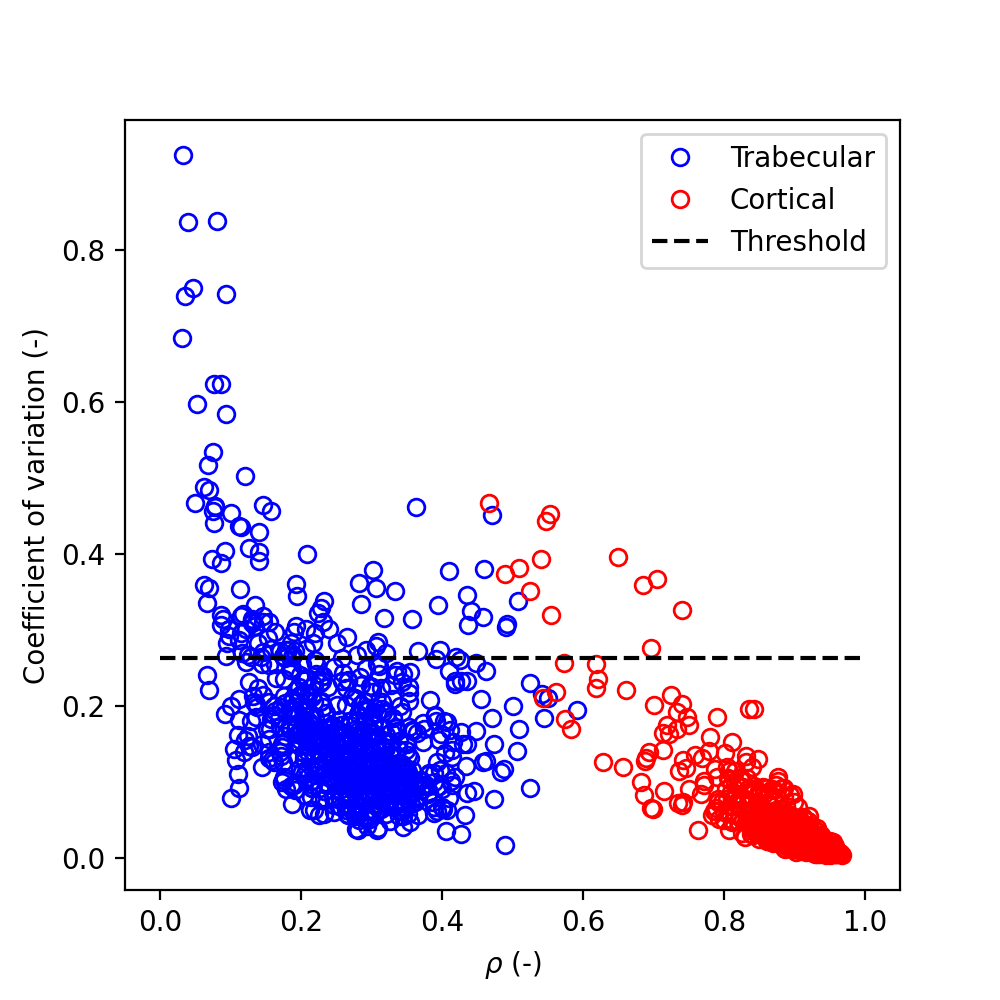
\includegraphics[width=\linewidth]{../Results/CV_Rho}
			\caption{Coefficient of variation as function of porosity}
	\end{figure}
	\begin{figure*}
		\centering
		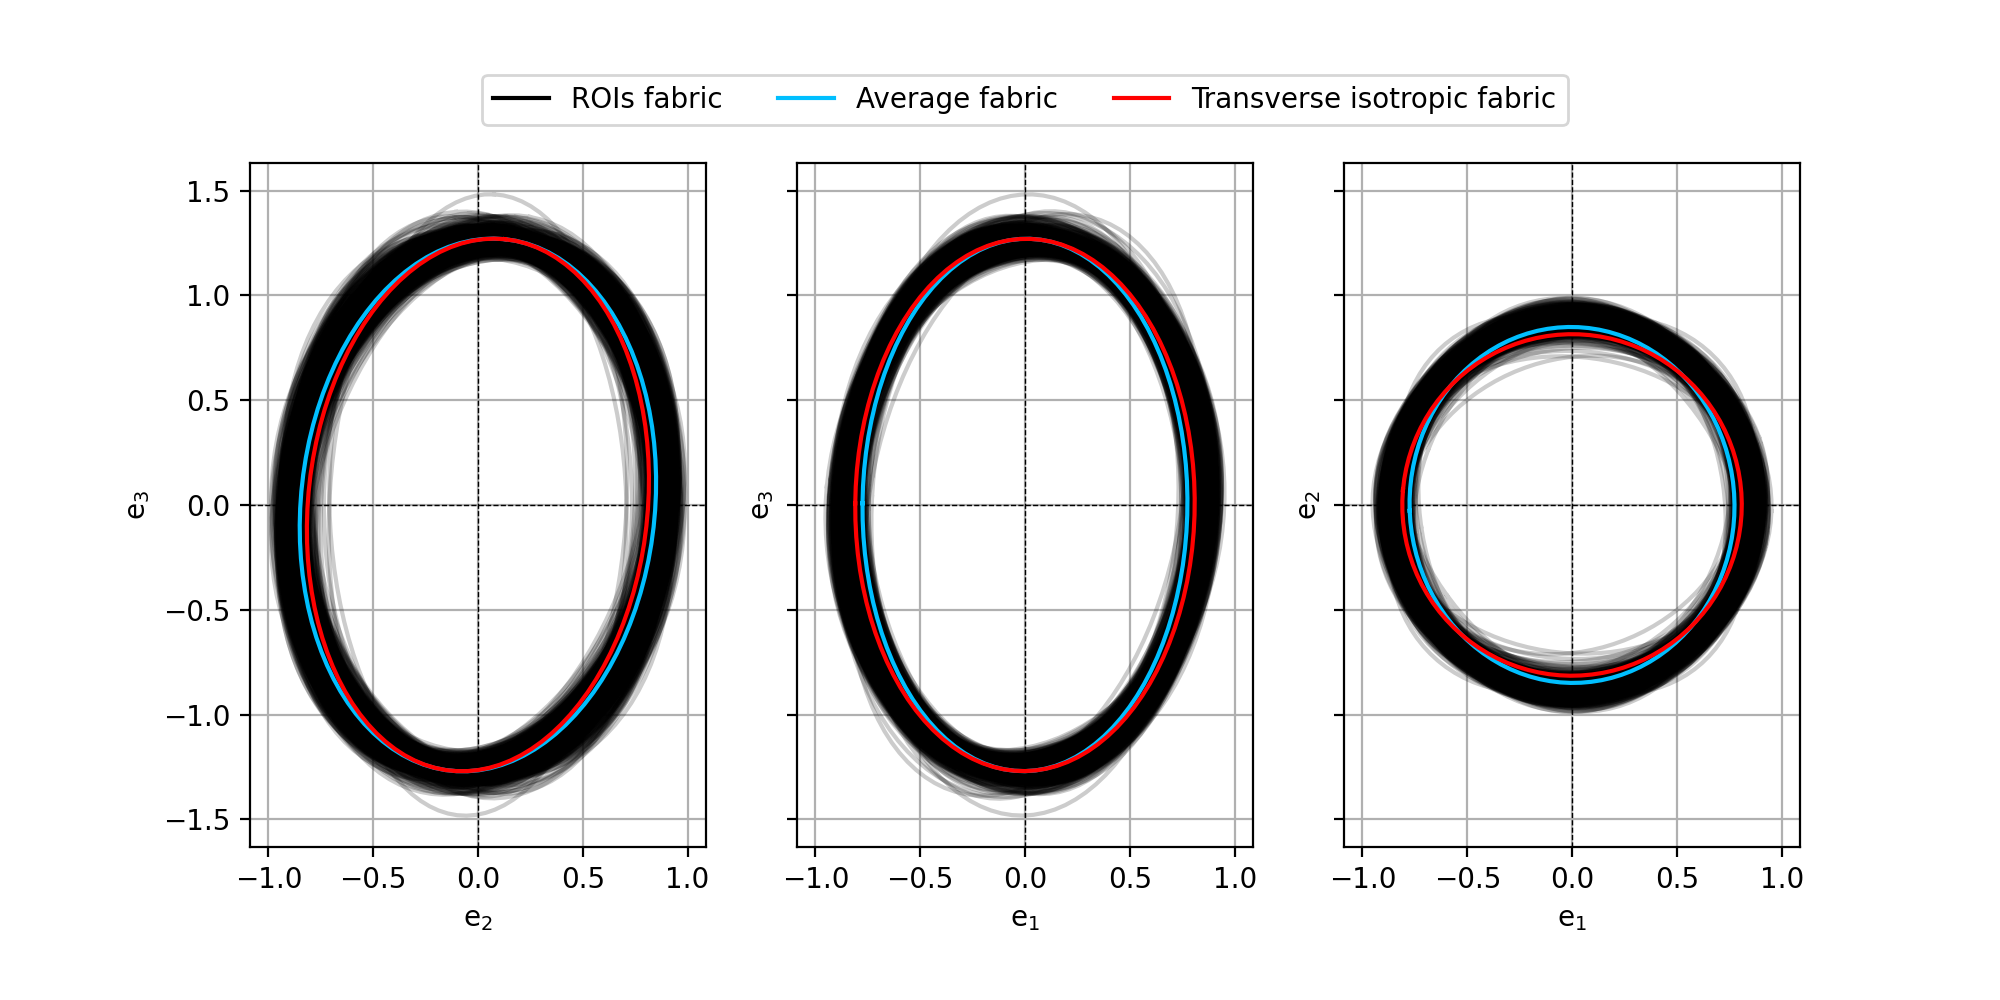
\includegraphics[width=\linewidth]{../Results/Fabric/Fabric}
		\caption{ROIs fabric projected on principal planes}
	\end{figure*}
	
	\clearpage
	\subsection{Fit to model}
	\begin{figure*}
		\centering
		\begin{subfigure}[t]{.3\linewidth}
			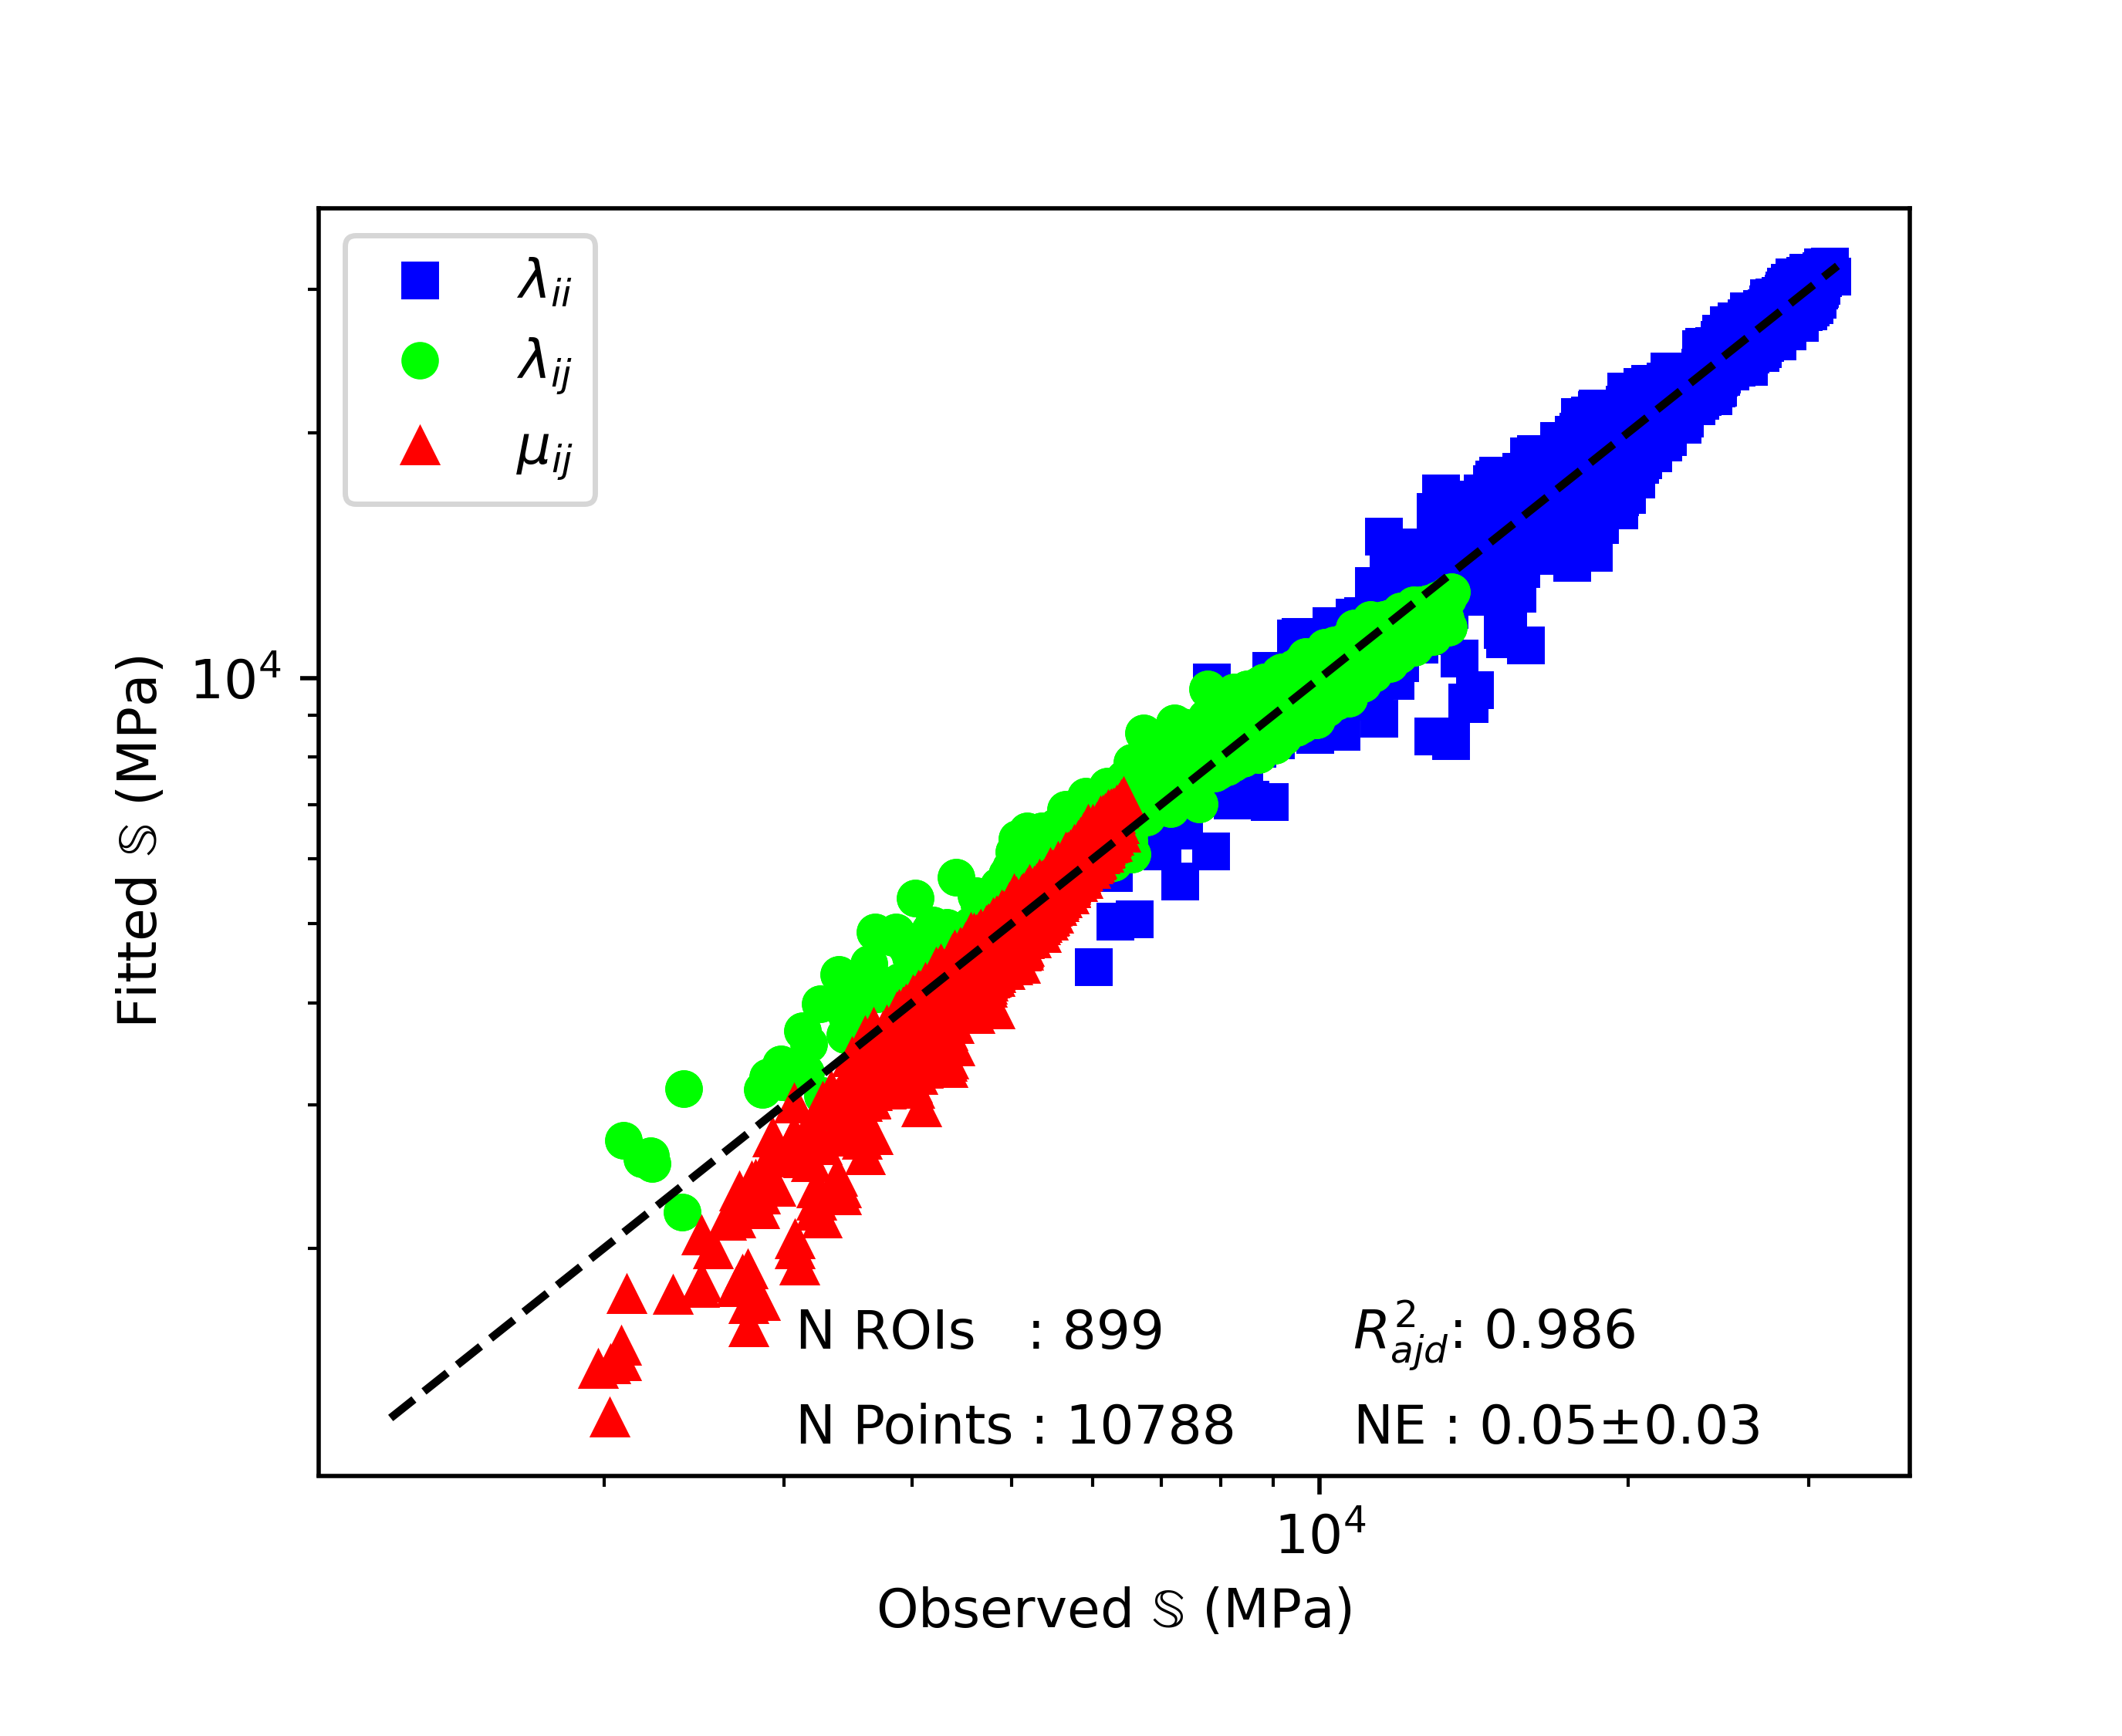
\includegraphics[height=0.8\linewidth]{../Results/StandardOrthoModel}
			\caption{Zysset-Curnier model in orthotropic space}
		\end{subfigure}
		\begin{subfigure}[t]{.3\linewidth}
			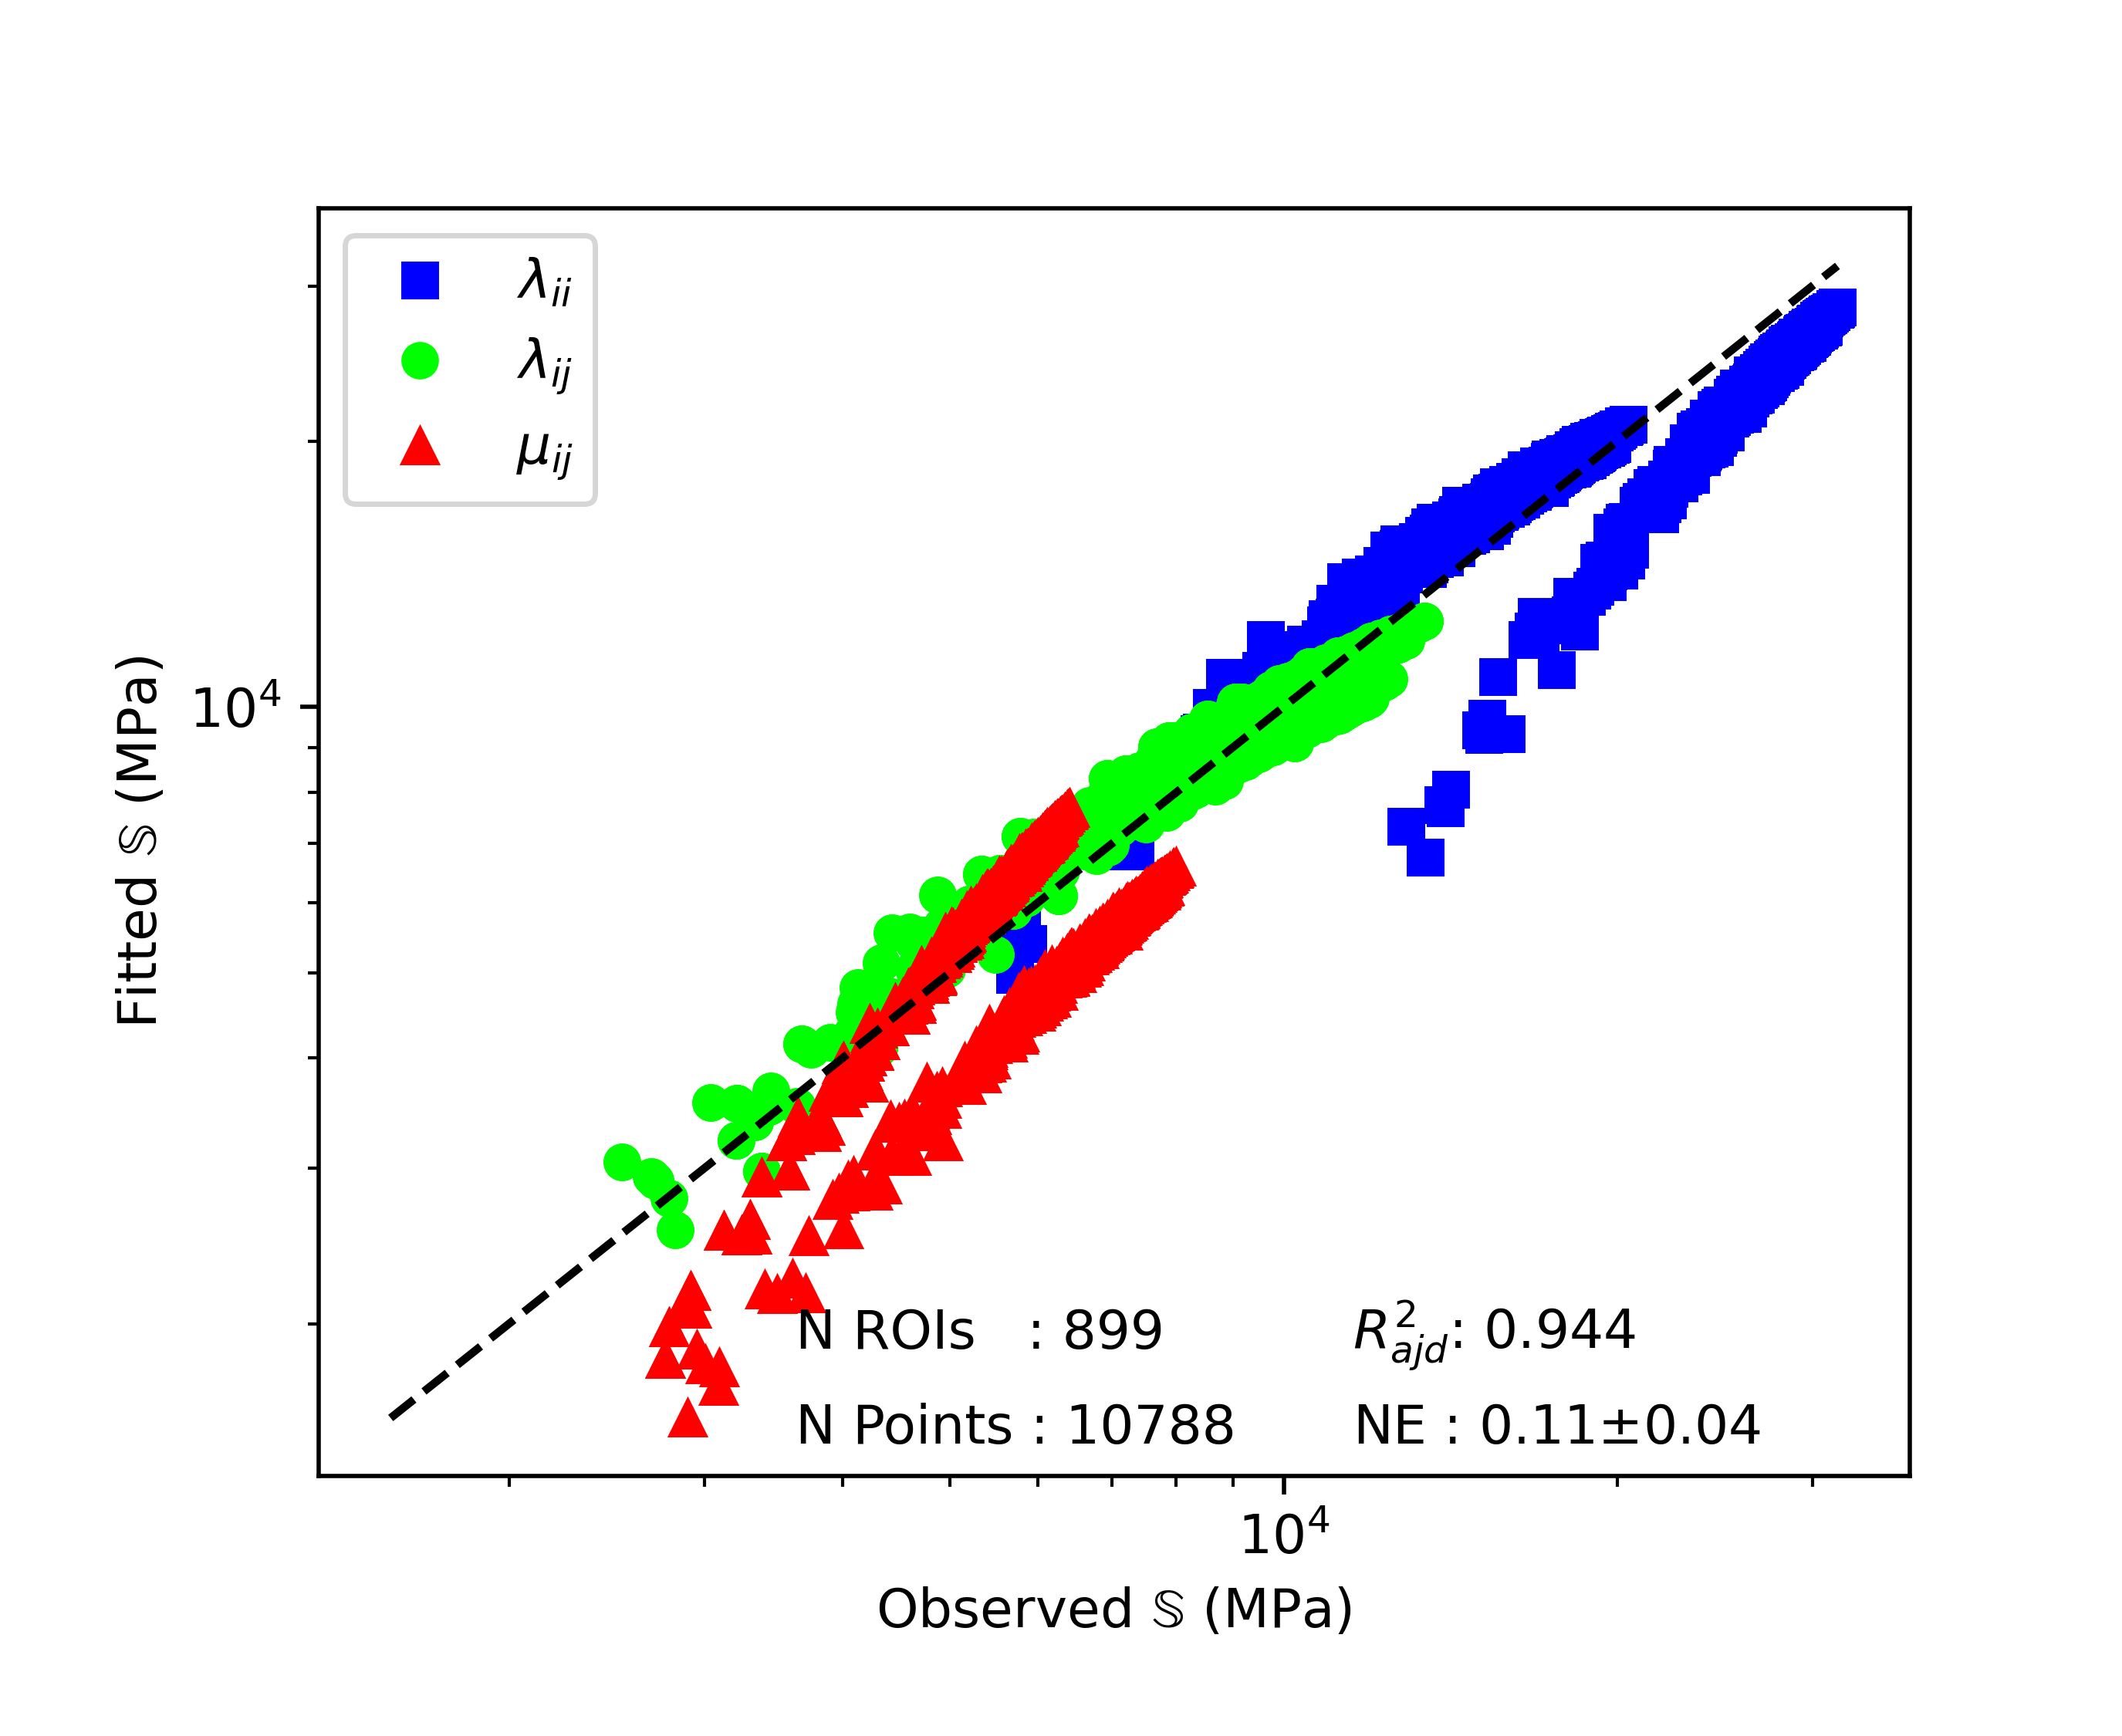
\includegraphics[height=0.8\linewidth]{../Results/StandardTransModel}
			\caption{Zysset-Curnier model in transverse isotropic space}
		\end{subfigure}
		\begin{subfigure}[t]{.3\linewidth}
			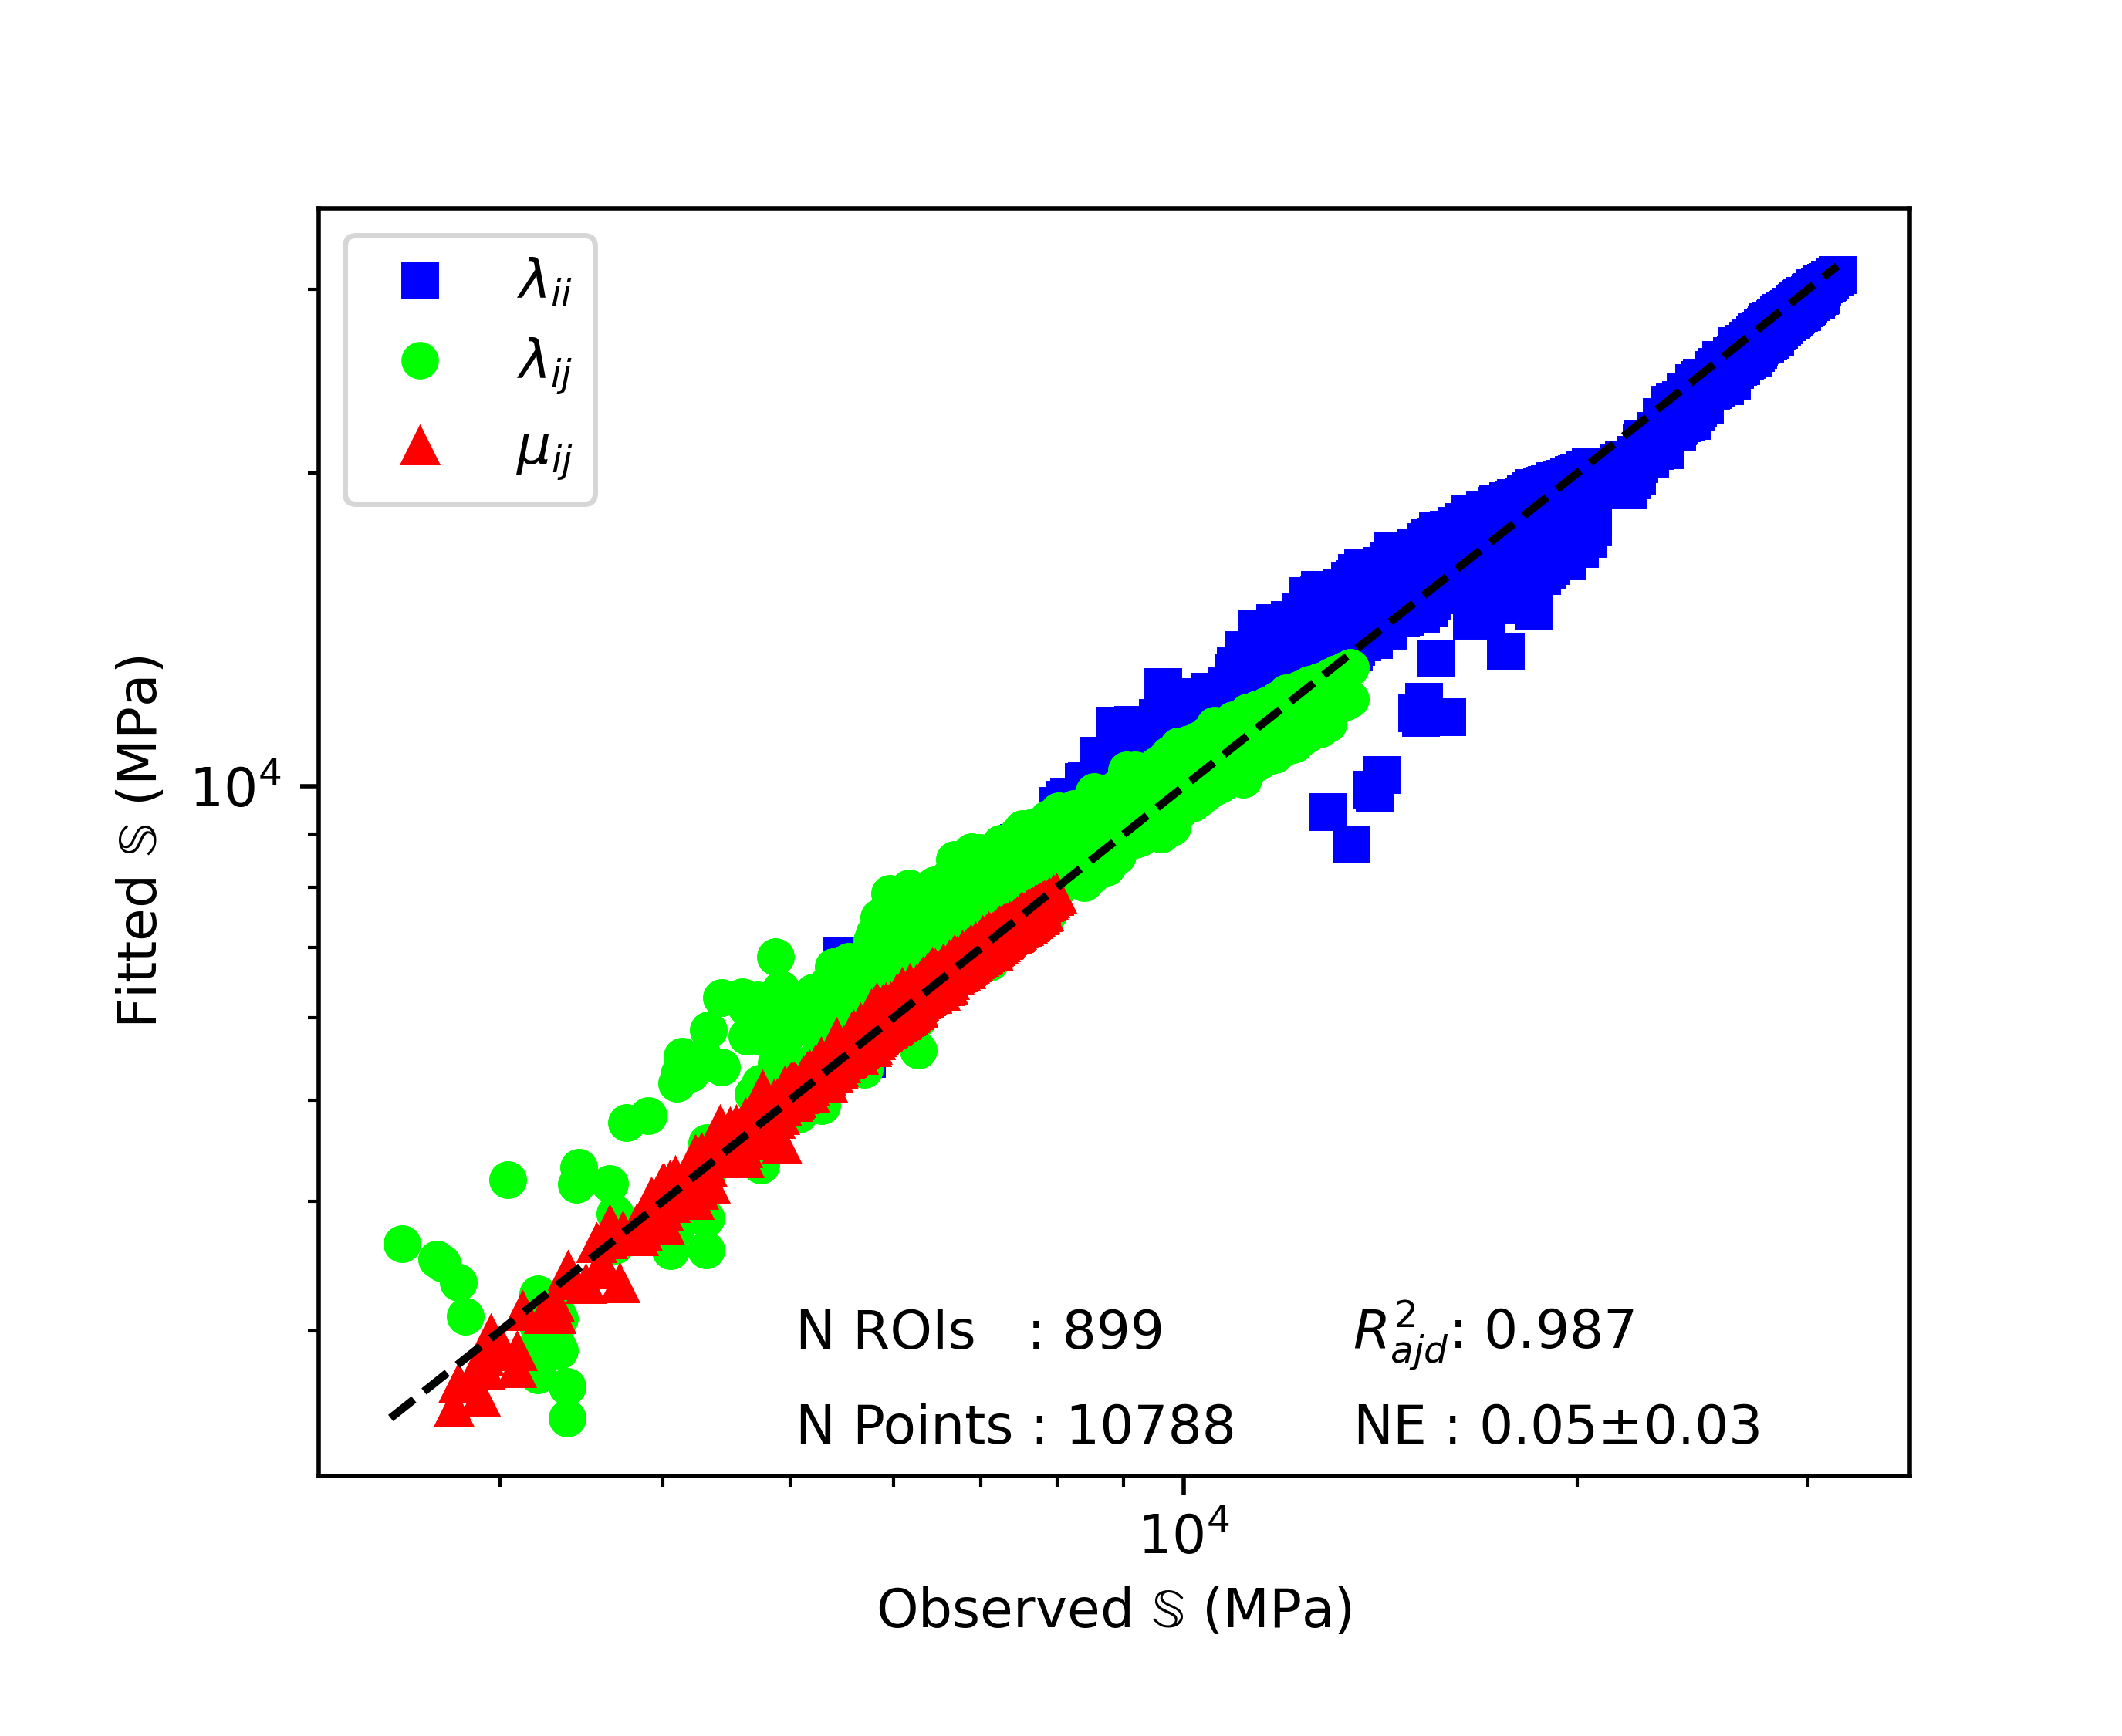
\includegraphics[height=0.8\linewidth]{../Results/SpectralModel}
			\caption{Yang and Cowin model in transverse isotropic space}
		\end{subfigure}
		\caption{Models fitting results}
	\end{figure*}
	\begin{table}[!h]
		\centering
		\caption{Parameters and fit quality coefficient obtained with the standard Zysset-Curnier model in orthotropic and transverse isotropic space.}
		\label{TabZysset}
		\begin{tabular}{l|c|c|c|c|c|c|c}
		\toprule
			Model & $\lambda_0$ & $\lambda_0'$ & $\mu_0$ &  $k$ &  $l$ & $R^2_{adj}$ &   NE \\
		\midrule
		Orthotropic &       19831 &        12618 &    3527 & 2.48 & 0.57 &        0.99 & 0.05 \\
		Transverse &       17505 &        13117 &    4016 & 2.49 & 0.39 &        0.94 & 0.11 \\
		\bottomrule
		\end{tabular}
	\end{table}

	\begin{figure*}
		\centering
			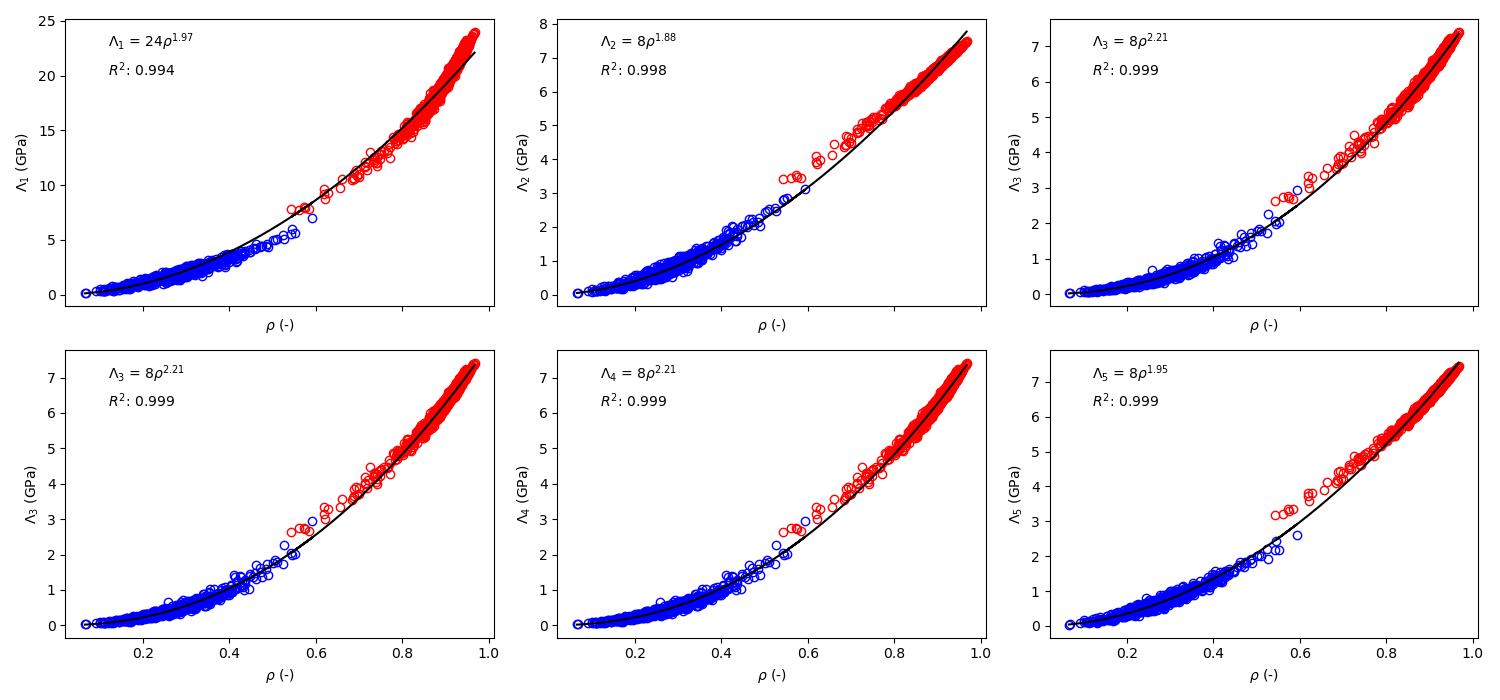
\includegraphics[width=\linewidth]{../Trabecular/LambdaVSRho}
			\caption{Eigenvalues of the stiffness tensor as function of porosity}
	\end{figure*}

	\begin{figure*}
		\centering
			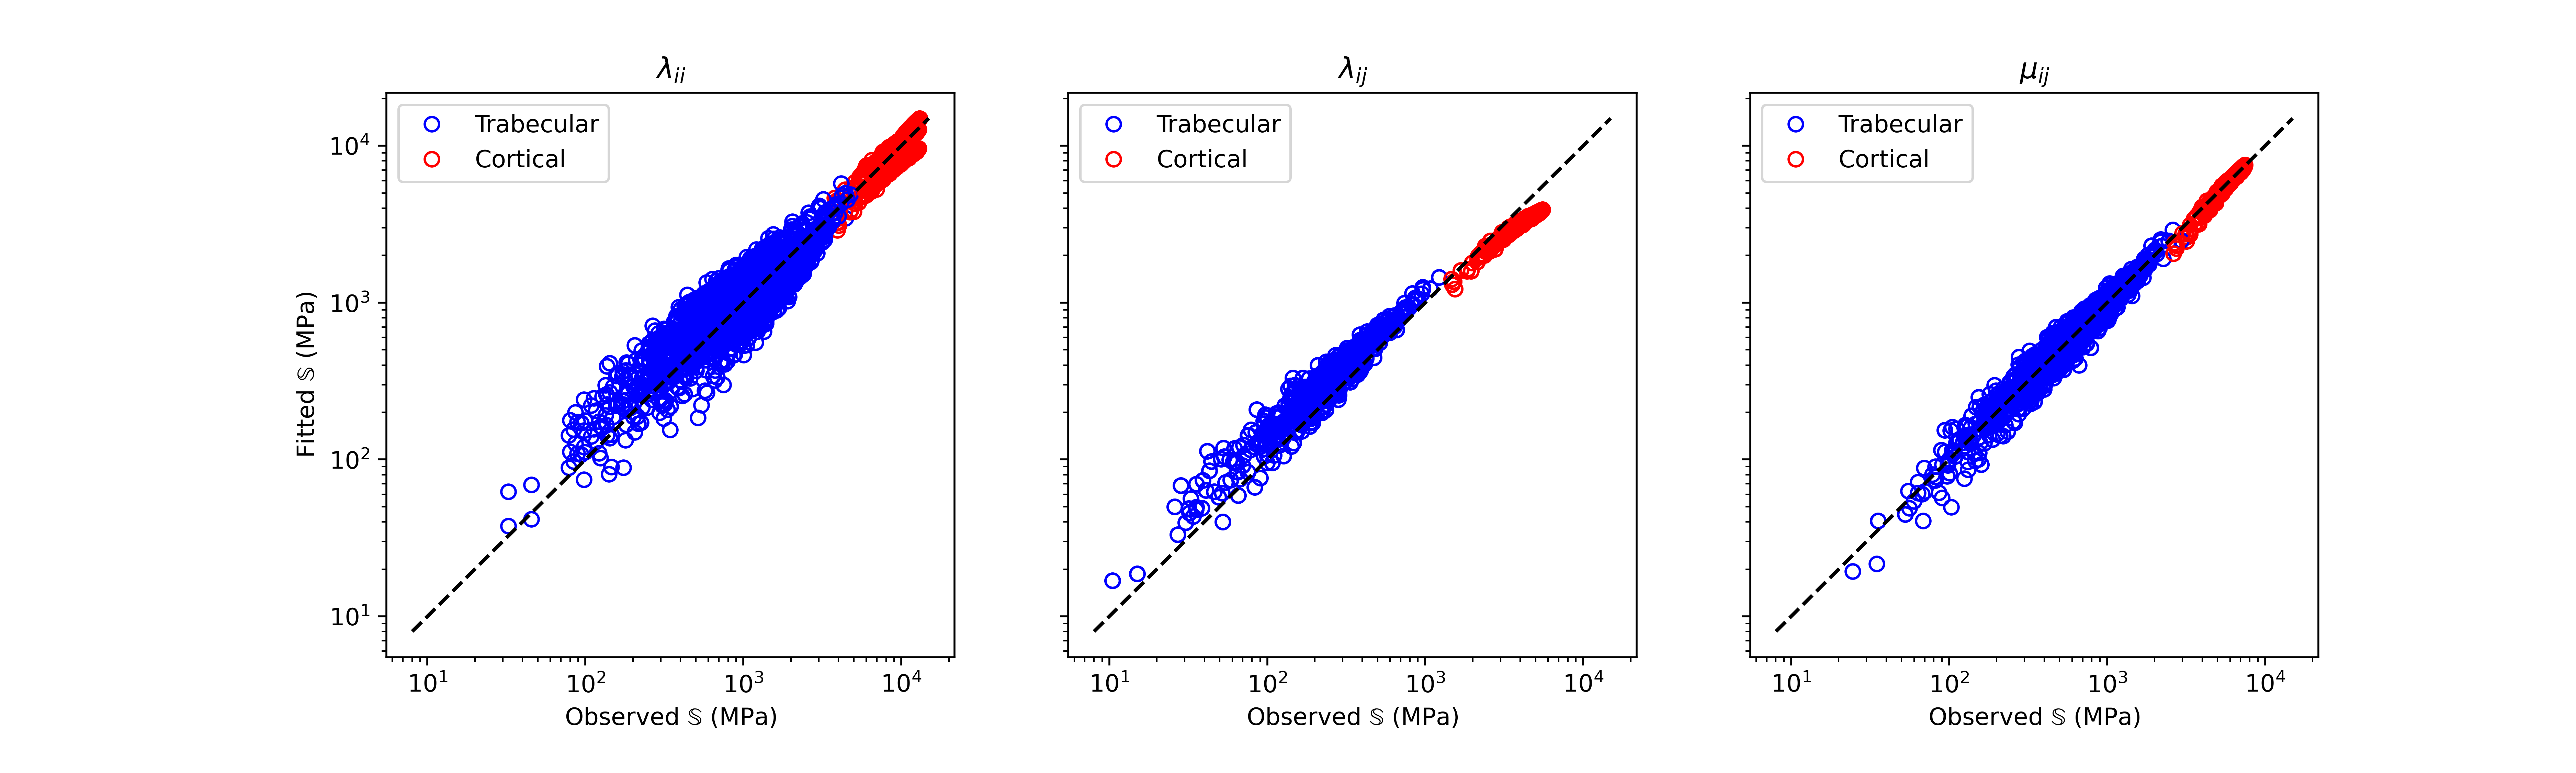
\includegraphics[width=\linewidth, trim= 100 0 100 0]{../Trabecular/SpectralModel}
			\caption{Result of fitting to Yang and Cowin model}
	\end{figure*}

	\clearpage
	\subsection{Comparison to RUS}

	\begin{figure}[!h]
		\centering
			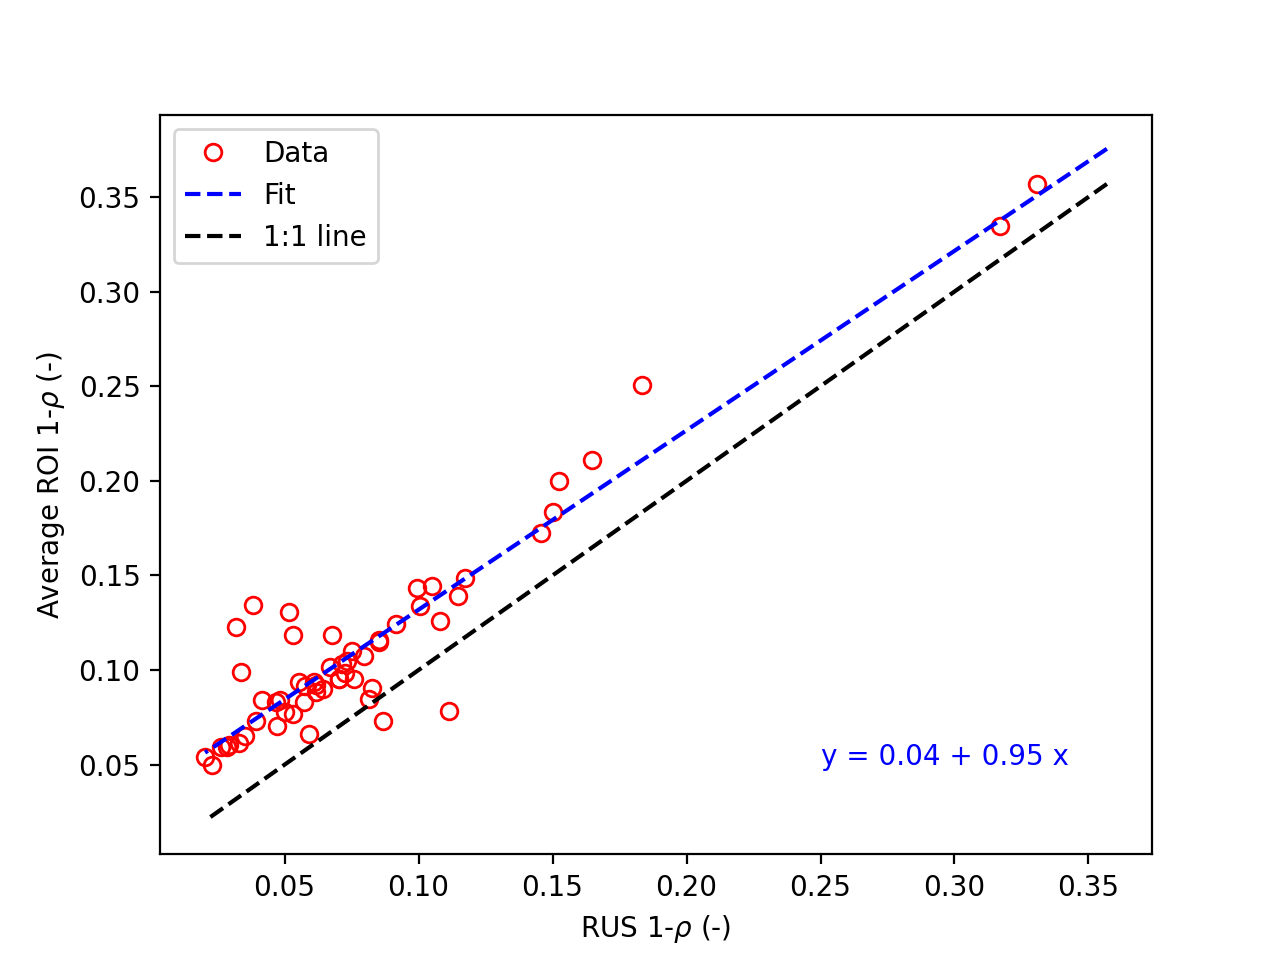
\includegraphics[height=\linewidth]{../Results/ExpSim_Rho}
			\caption{Average ROI porosity vs porosity from Cai et al.}
	\end{figure}

	\begin{figure*}[!h]
		\centering
		\begin{subfigure}[t]{.3\linewidth}
		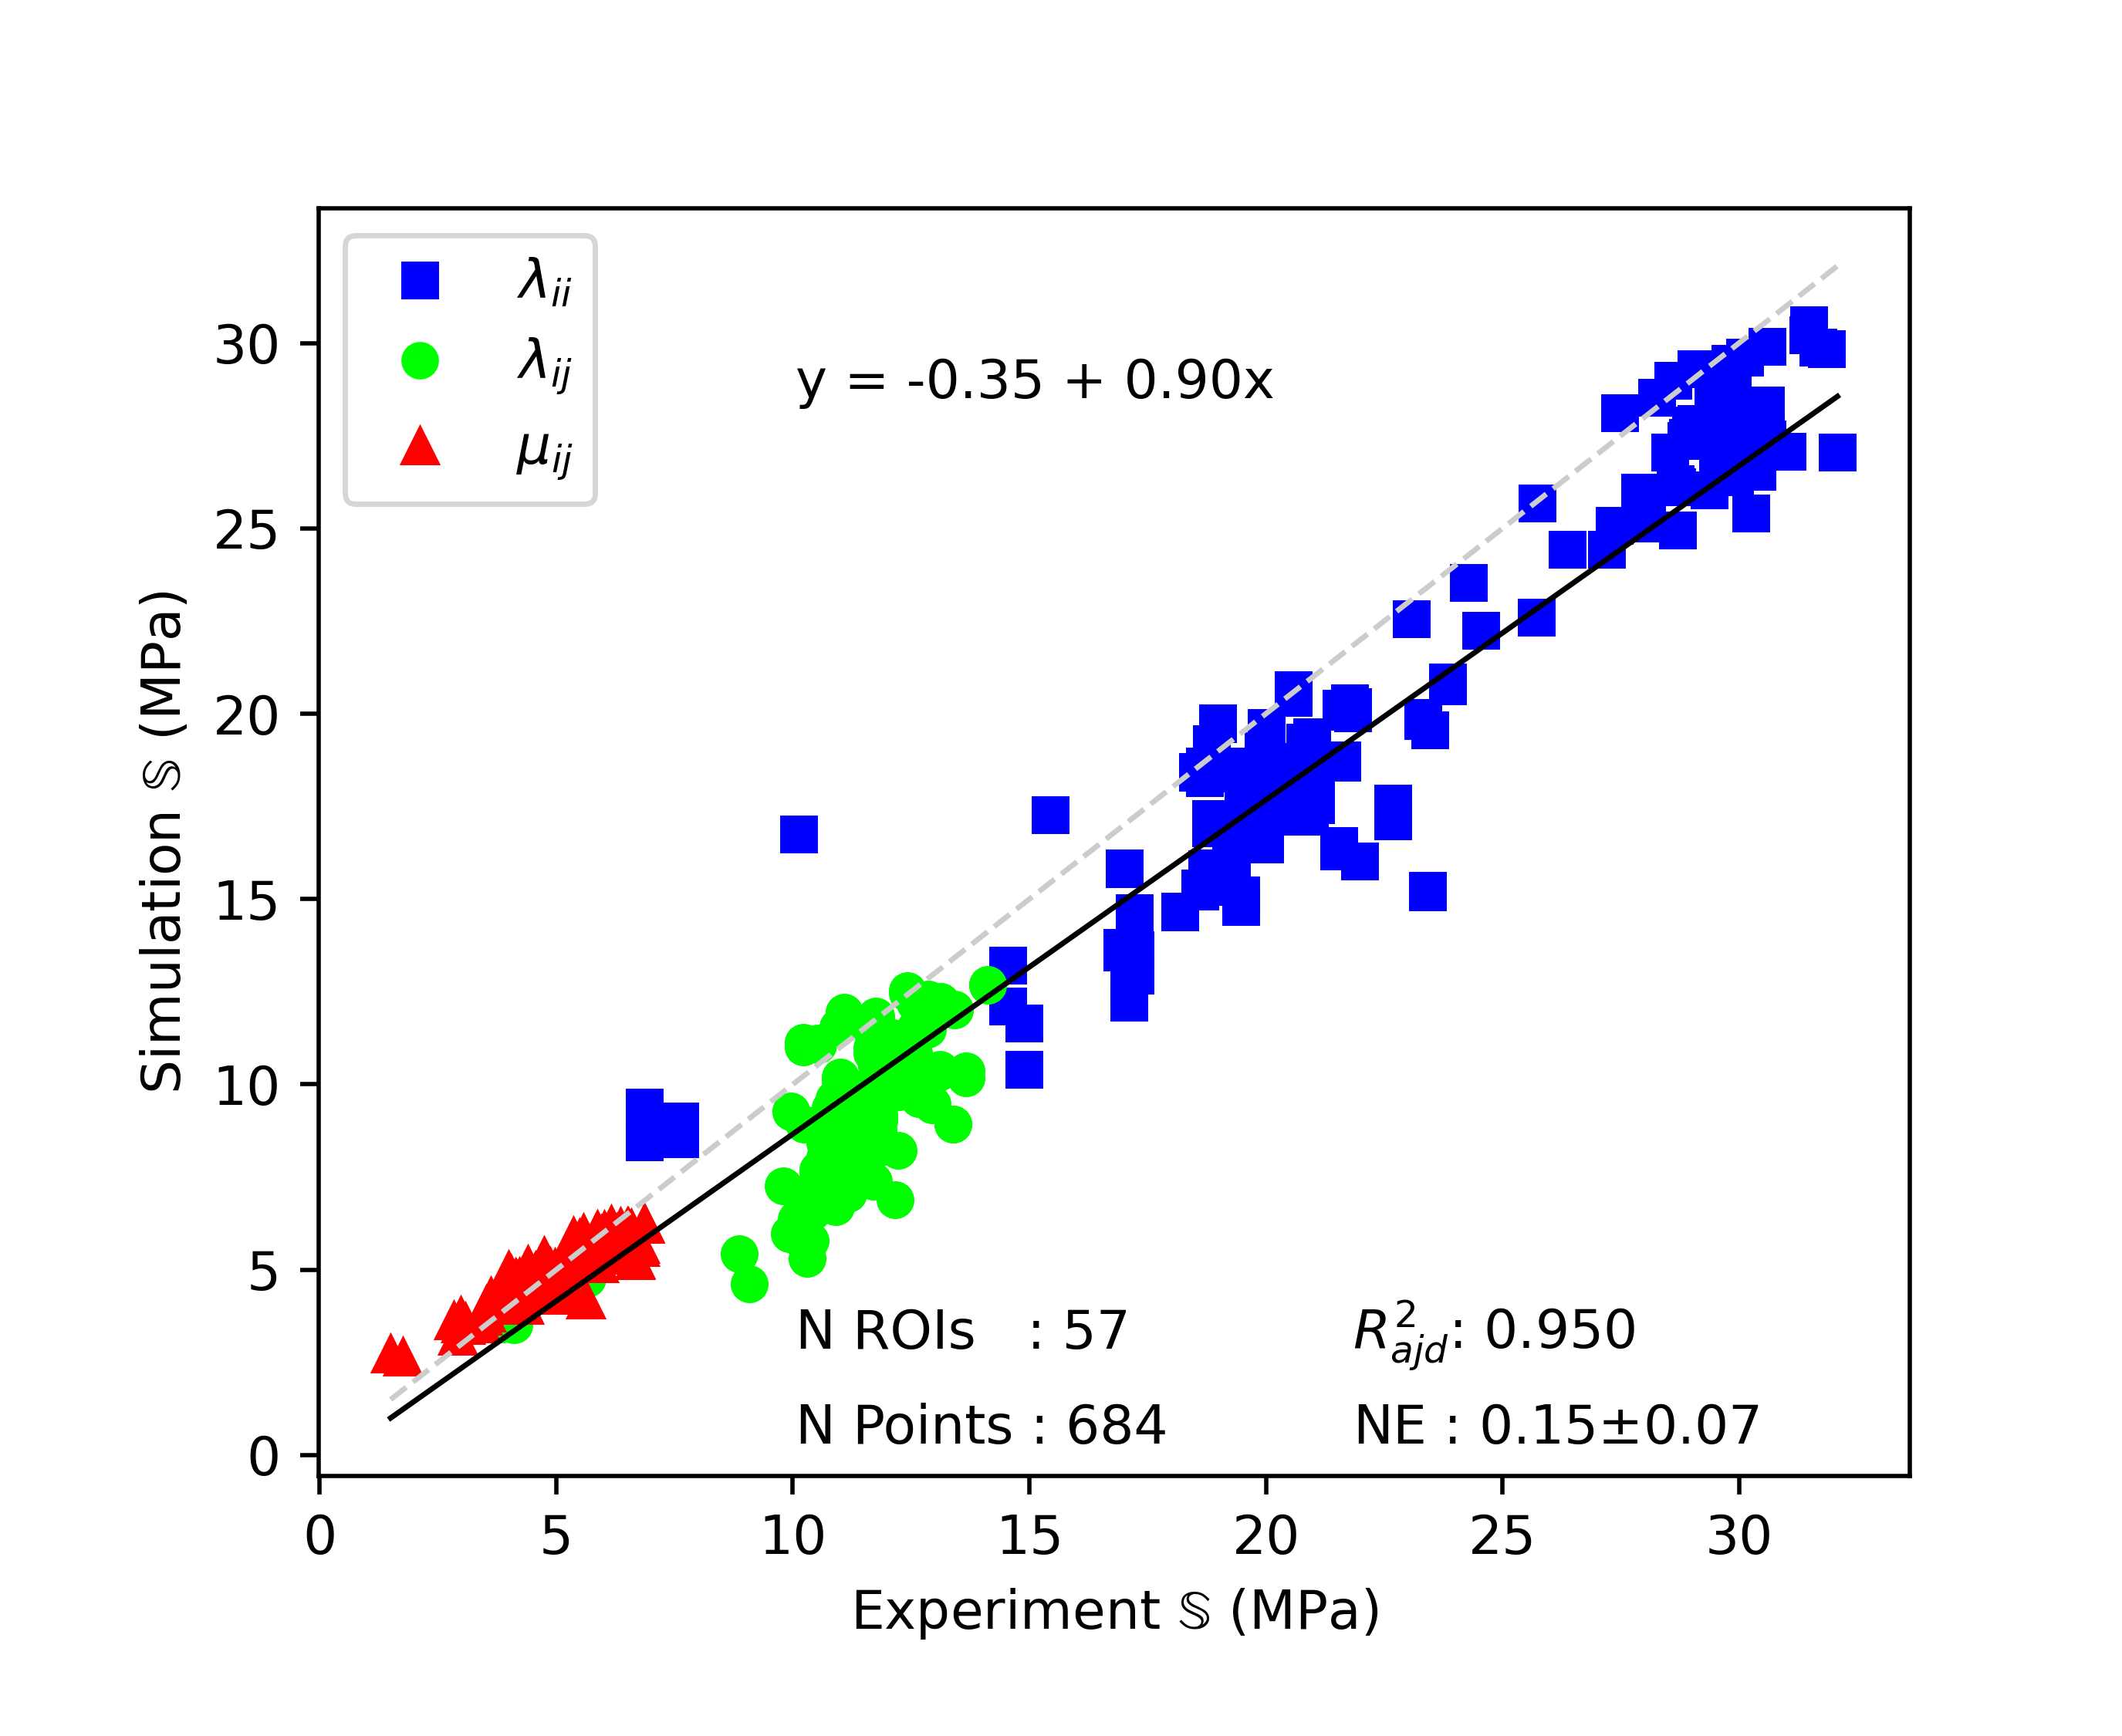
\includegraphics[height=0.8\linewidth]{../Results/ExpSim_S_Raw}
		\caption{Orthotropic space}
		\end{subfigure}
		\begin{subfigure}[t]{.3\linewidth}
		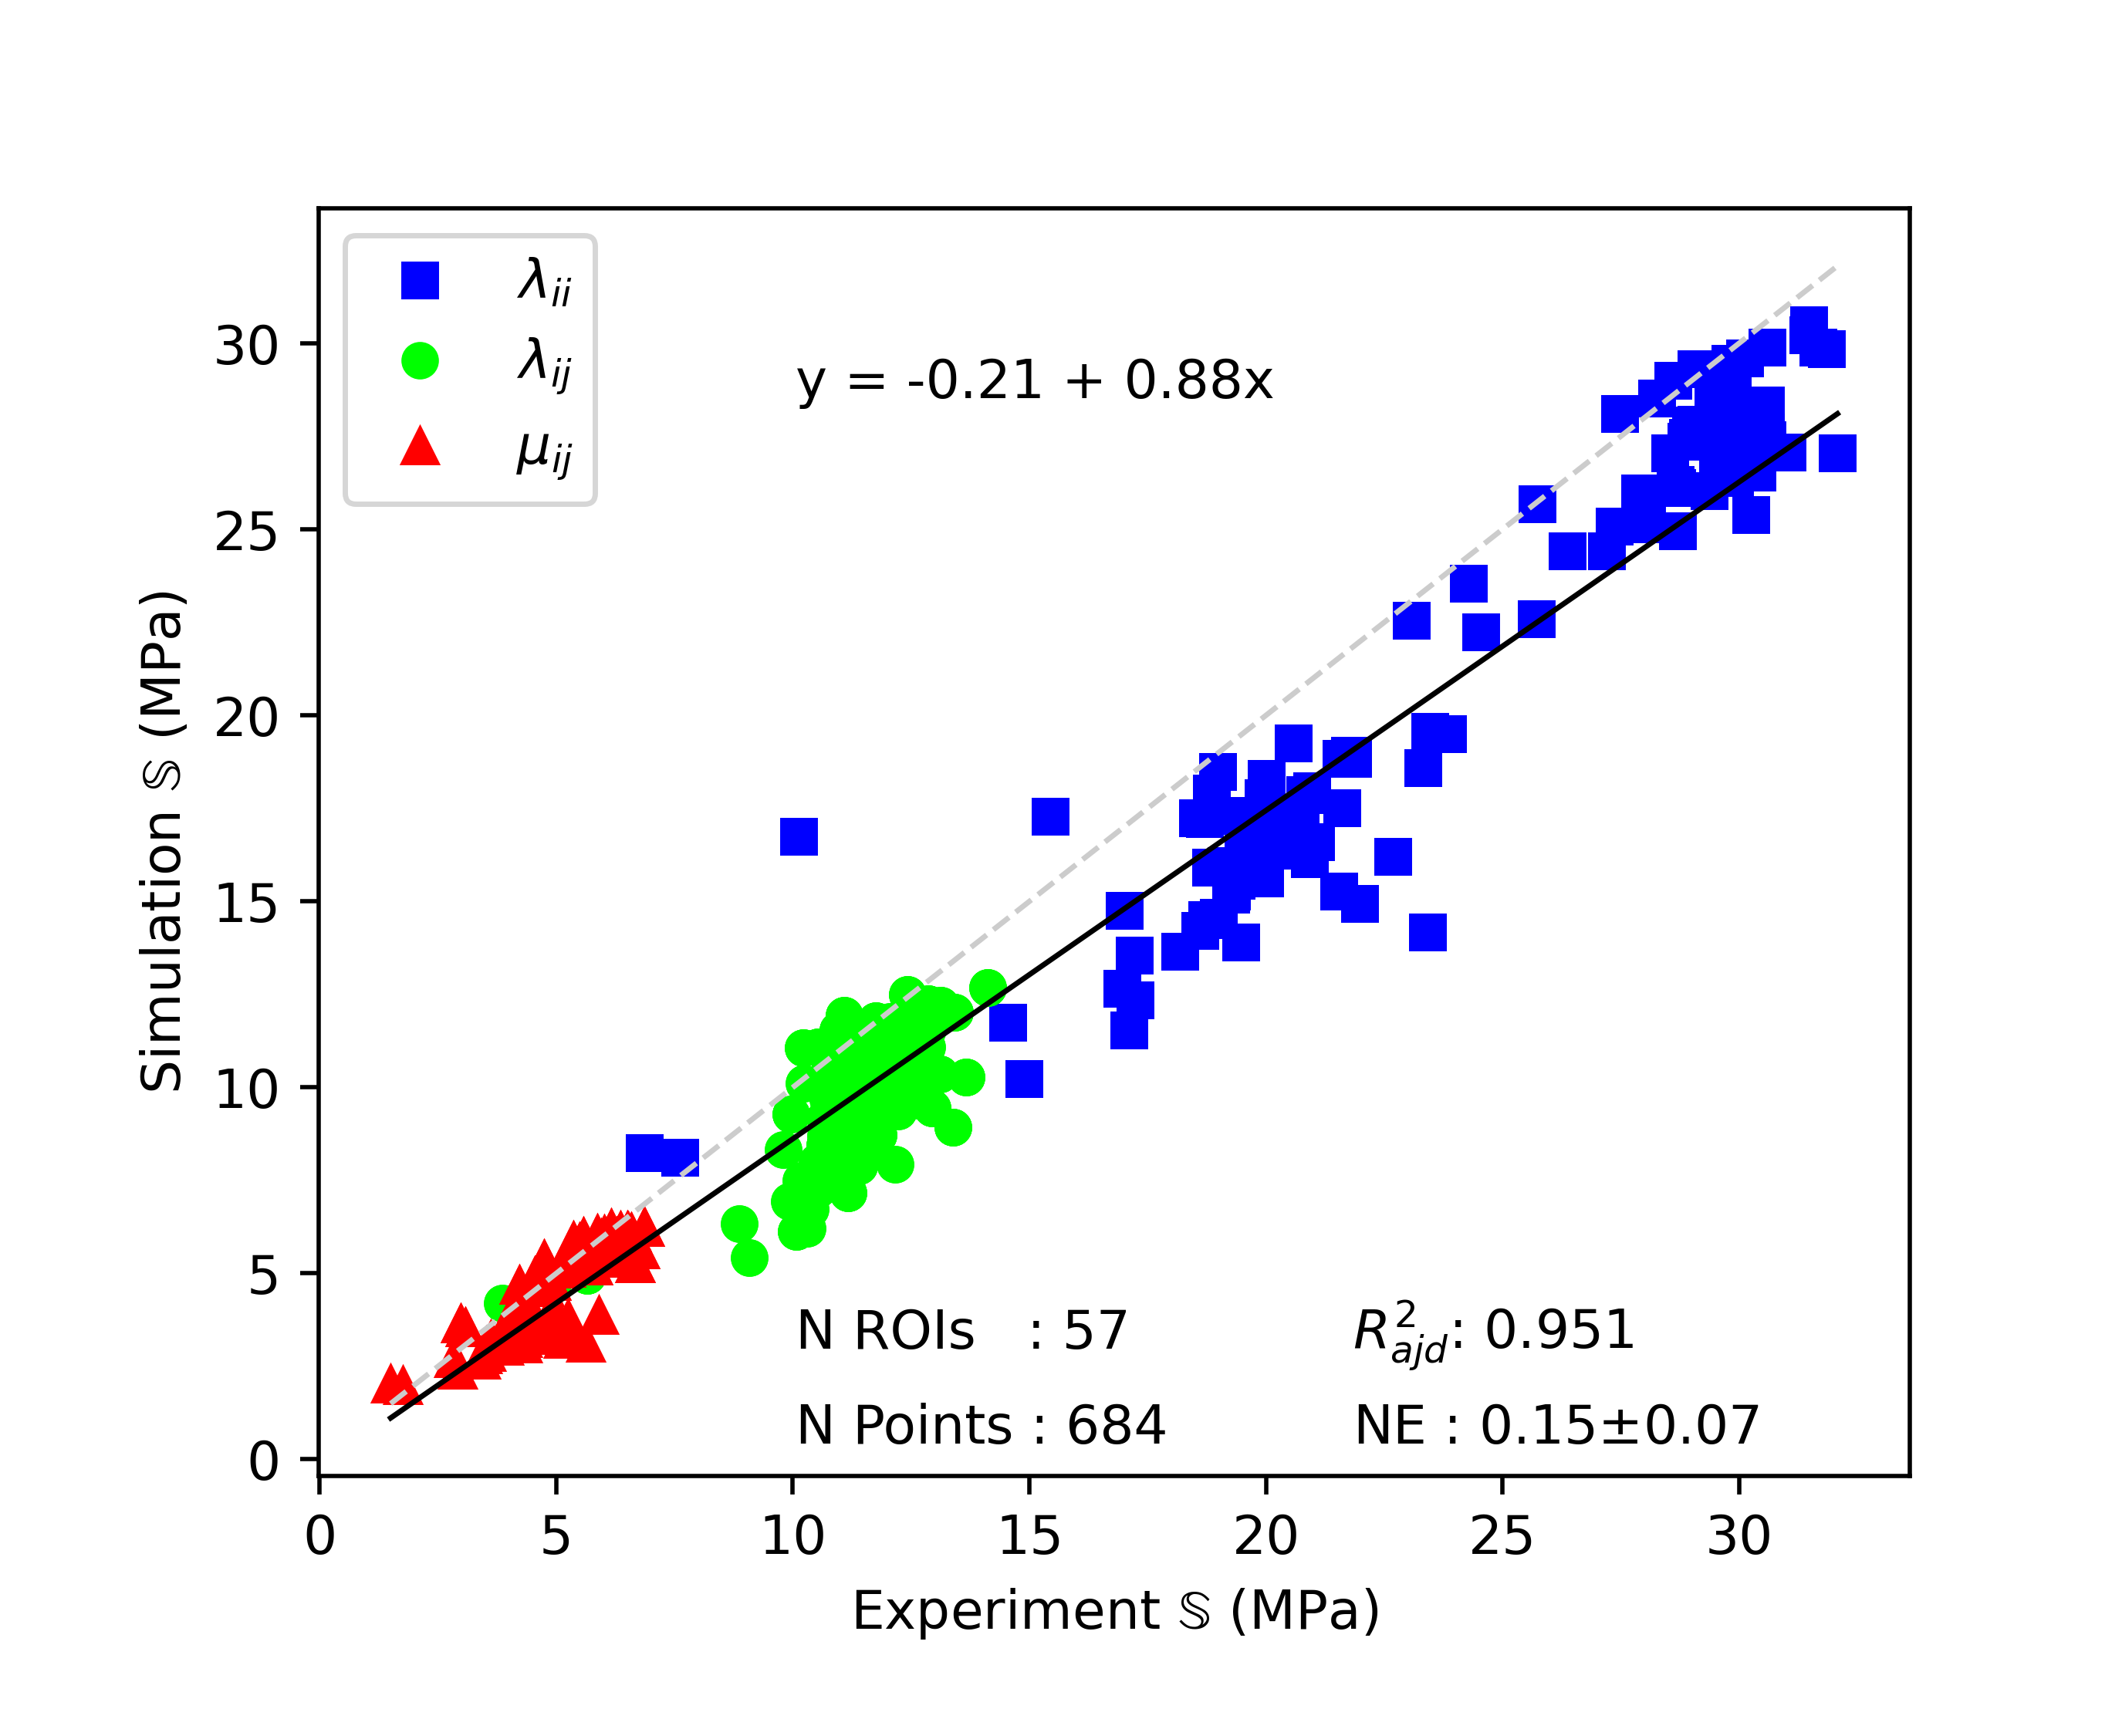
\includegraphics[height=0.8\linewidth]{../Results/ExpSim_S_Proj}
		\caption{Transverse isotropic space}
		\end{subfigure}
		\begin{subfigure}[t]{.3\linewidth}
		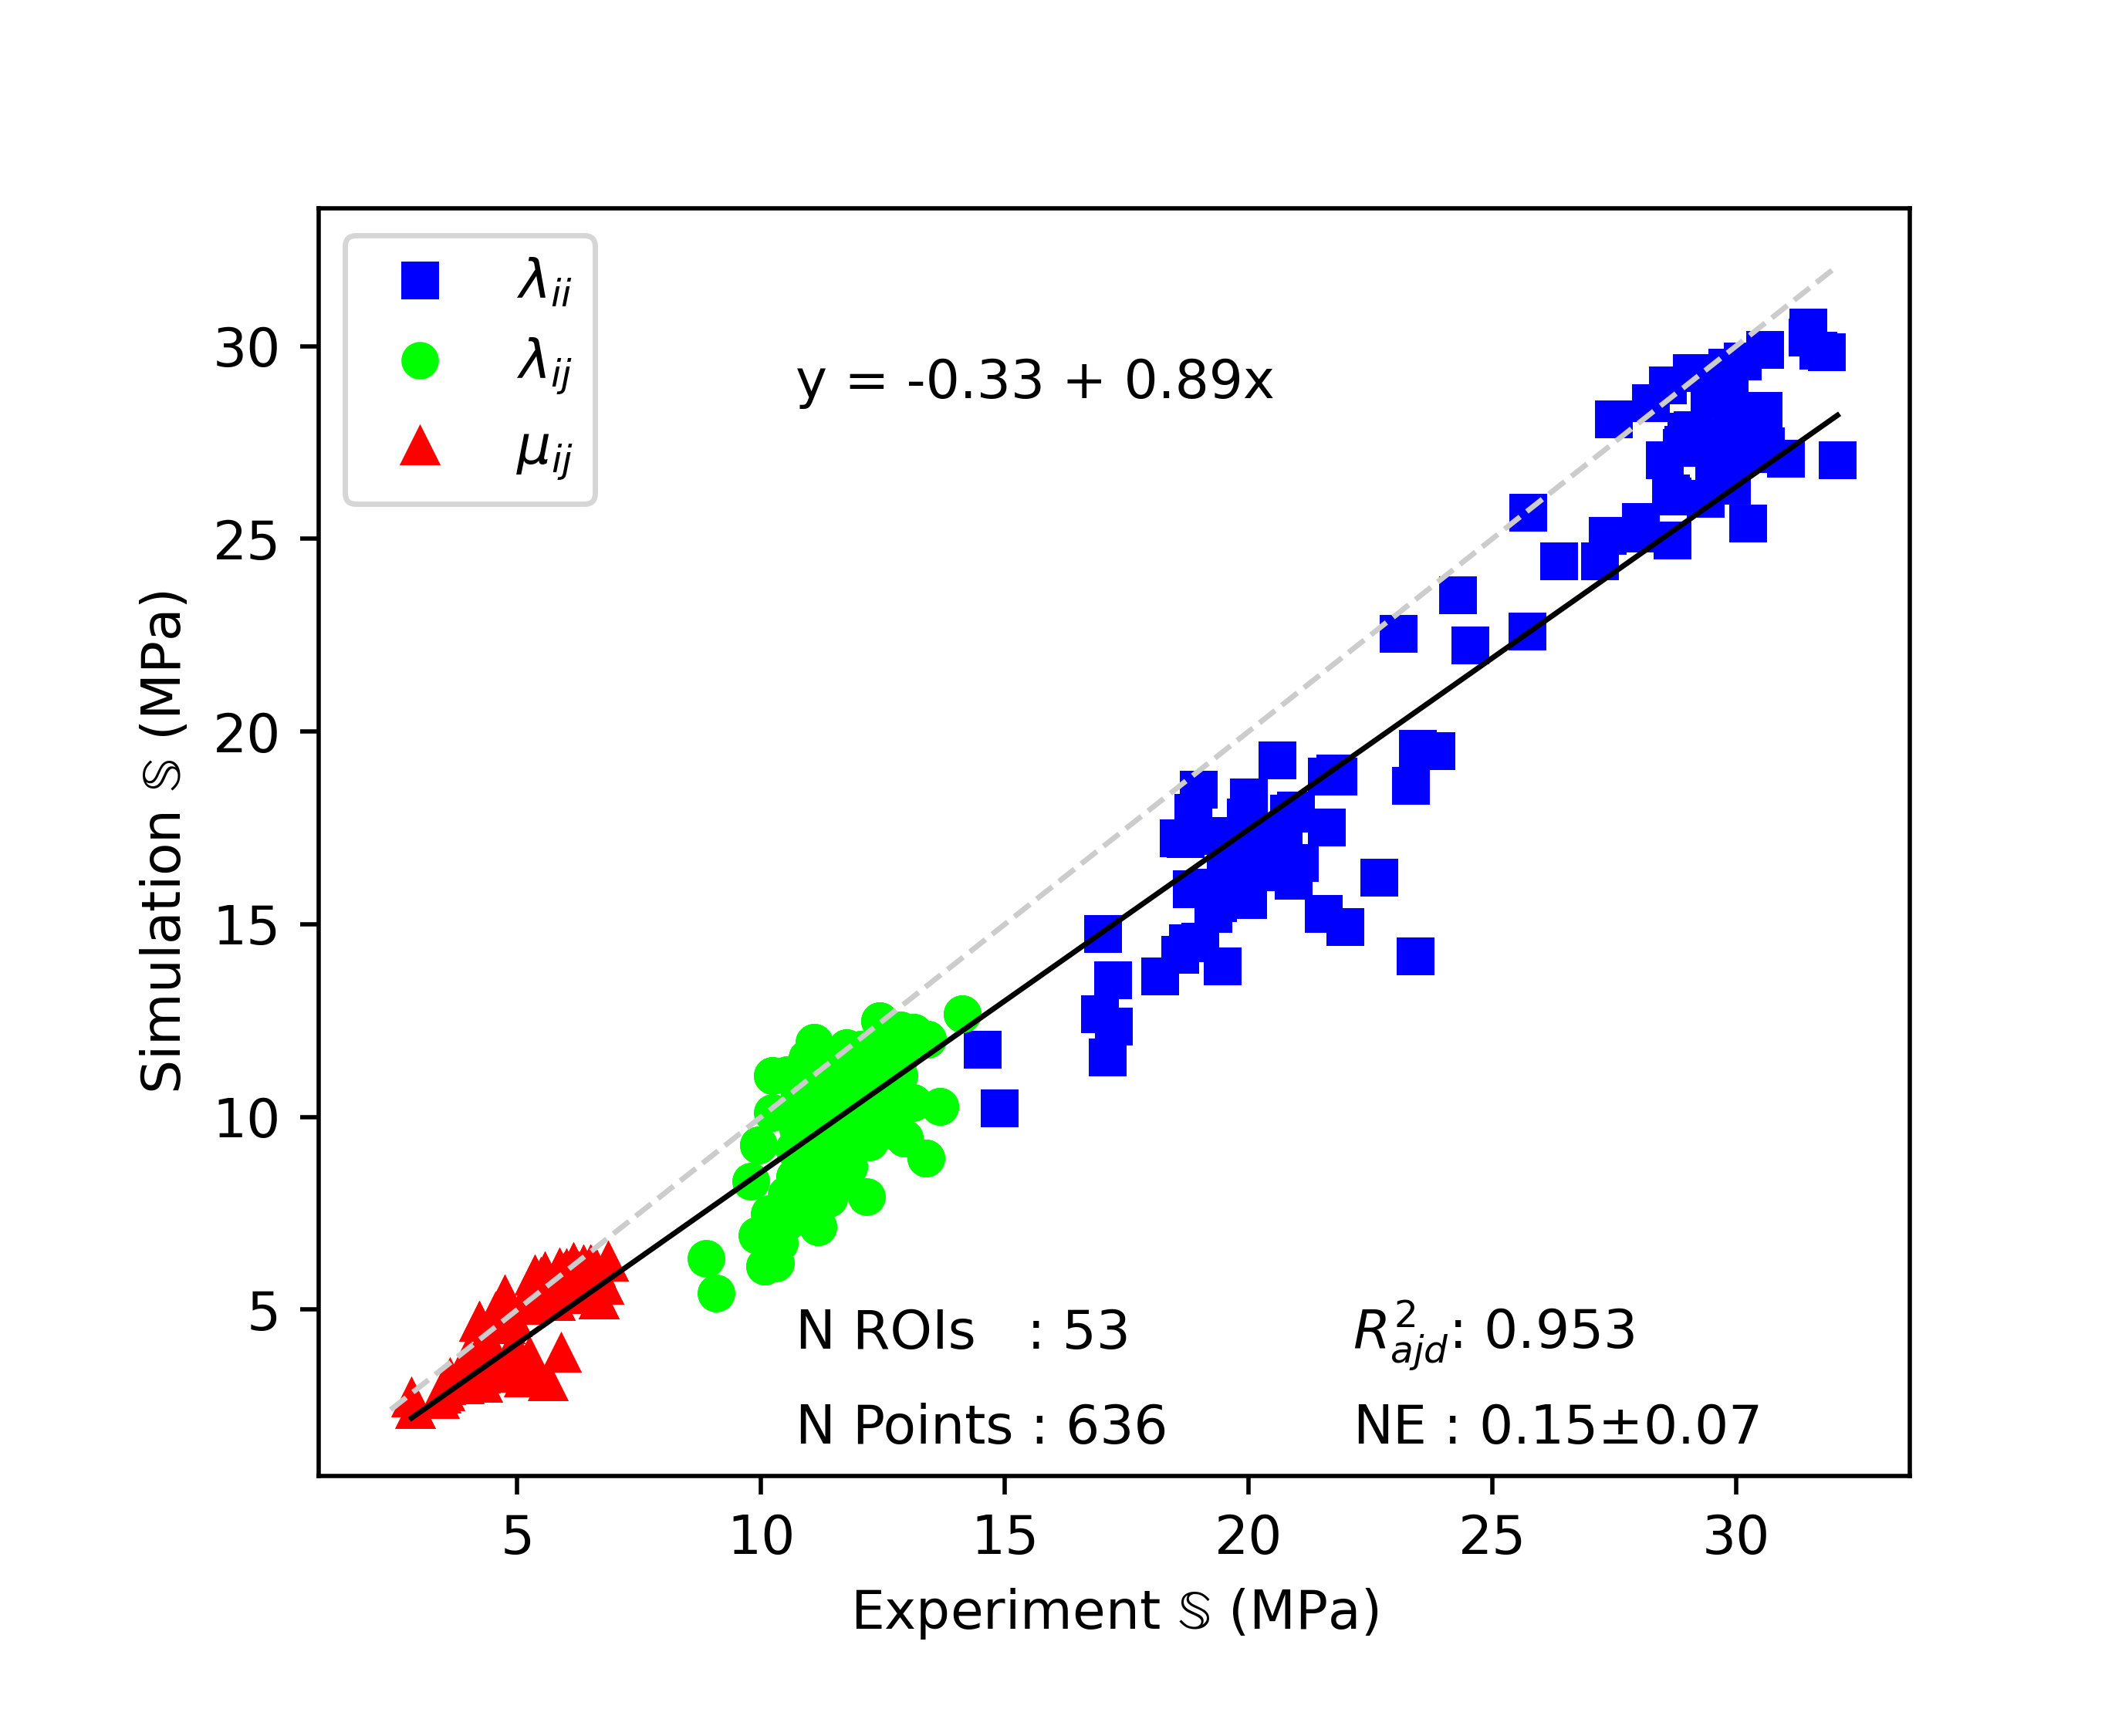
\includegraphics[height=0.8\linewidth]{../Results/ExpSim_S_Filt}
		\caption{Transverse isotropic space, high CV filtered}
		\end{subfigure}		
		\caption{Simulation vs experimental stiffness tensor components}
	\end{figure*}

	\begin{figure*}
		\centering
		\begin{subfigure}[b]{0.45\linewidth}
			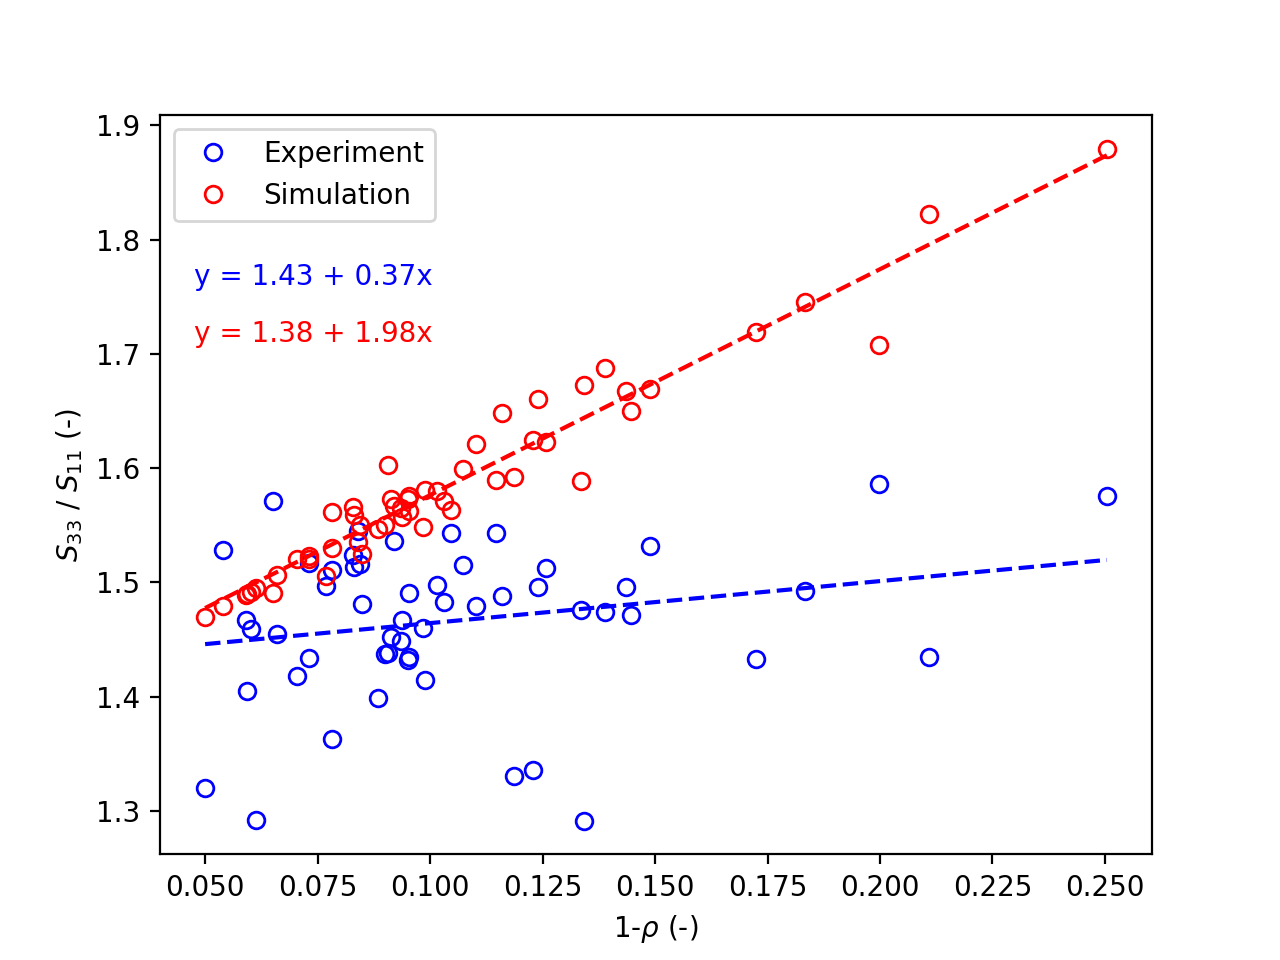
\includegraphics[width=\linewidth]{../Results/ExpSim_AniS}
			\caption{Stiffness ratio}
		\end{subfigure}
		\begin{subfigure}[b]{0.45\linewidth}
			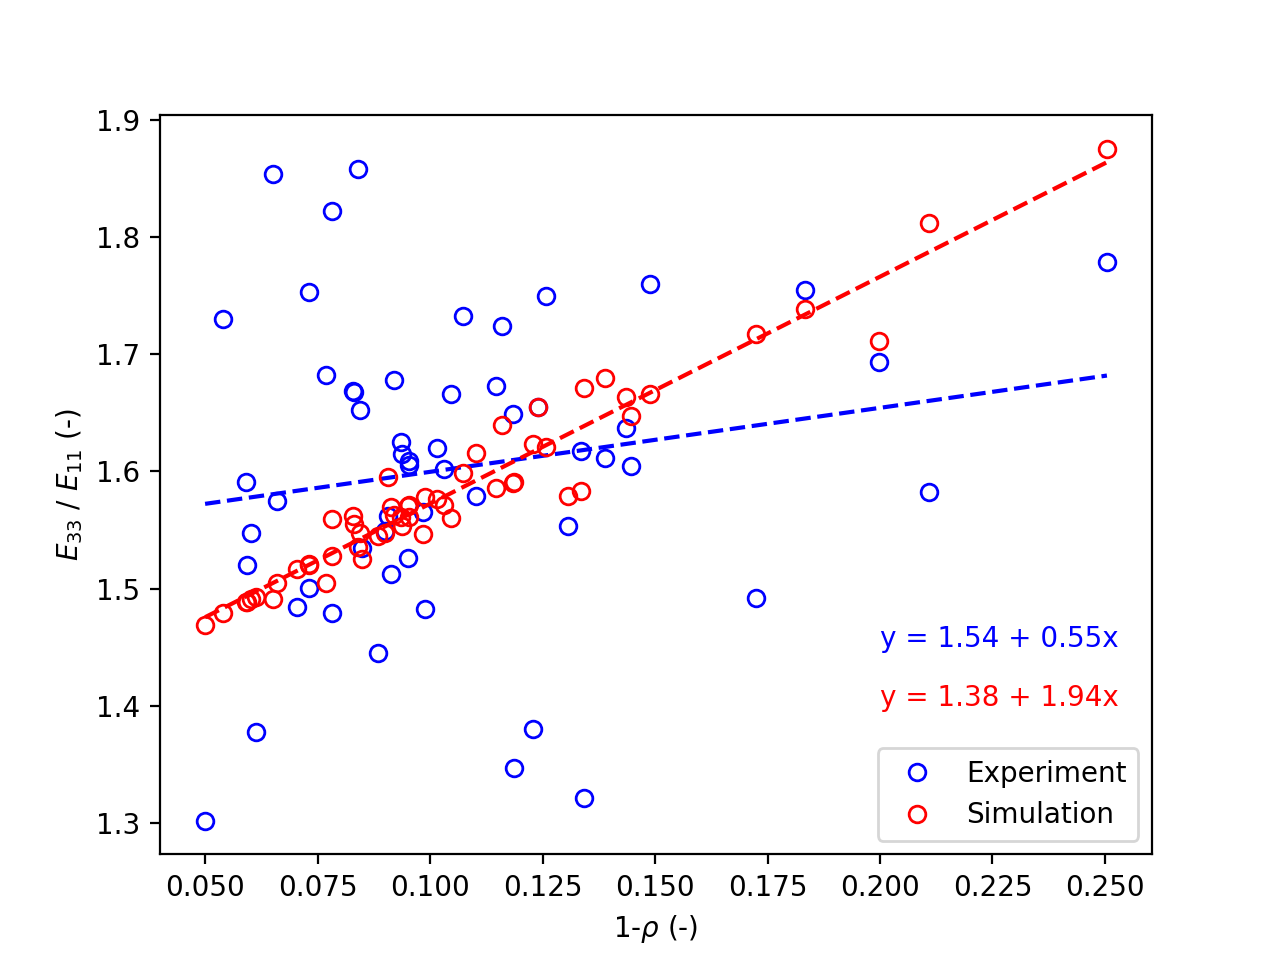
\includegraphics[width=\linewidth]{../Results/ExpSim_AniE}
			\caption{Young's moduli ratio}
		\end{subfigure}
		\caption{Degree of anisotropy}
	\end{figure*}

	%
	%
	%
	% DISCUSSION
	%
	%
	%
	
	\clearpage
	\section{Discussion and Conclusion}
	
	%
	%
	%
	% ACKNOWLEGMENTS
	%
	%
	%
	
	\section*{Declaration of competing interest}
	We wish to confirm that there are no known conflicts of interest associated with this publication and there has been no significant financial support for this work that could have influenced its outcome.
	
	\section*{Funding}
	This work was funded by the Swiss National Science Foundation (SNSF), grant number 200365.

	\section*{Data availability statement}
	The data that support the findings of this study are available on request. The data are not publicly available due to privacy/ethical restrictions. The scripts used for the analyses performed in the present study are available on Github: \url{https://github.com/artorg-unibe-ch/FABTIB}
	
	\section*{Research ethics}
	We further confirm that any aspect of the work covered in this manuscript that has involved human patients has been conducted with the ethical approval of all relevant bodies and that such approvals are acknowledged within the manuscript.
	
	\section*{CRediT author statement}
	\textbf{Mathieu Simon:} Data Curation, Formal analysis, Investigation, Methodology, Software, Visualization, Writing - original draft.
	\textbf{Philippe Zysset:} Conceptualization, Funding acquisition, Methodology, Project administration, Resources, Supervision, Validation, Writing - review and editing.
	
	%
	%
	%
	% Bibliography
	%
	%
	%

	% \clearpage
	% Loading bibliography database
	\nocite{*}
	\bibliographystyle{BibStyle}
	\bibliography{Bibliography}

	% \bibliographystyle{elsarticle-num} 

	% \begin{thebibliography}{65}
	% \expandafter\ifx\csname natexlab\endcsname\relax\def\natexlab#1{#1}\fi
	% \providecommand{\url}[1]{\texttt{#1}}
	% \providecommand{\href}[2]{#2}
	% \providecommand{\path}[1]{#1}
	% \providecommand{\DOIprefix}{doi:}
	% \providecommand{\ArXivprefix}{arXiv:}
	% \providecommand{\URLprefix}{URL: }
	% \providecommand{\Pubmedprefix}{pmid:}
	% \providecommand{\doi}[1]{\href{http://dx.doi.org/#1}{\path{#1}}}
	% \providecommand{\Pubmed}[1]{\href{pmid:#1}{\path{#1}}}
	% \providecommand{\bibinfo}[2]{#2}
	% \ifx\xfnm\relax \def\xfnm[#1]{\unskip,\space#1}\fi
	% %Type = Article
	% \bibitem[{Bala and Seeman(2015)}]{Bala2015}
	% \bibinfo{author}{Bala, Y.}, \bibinfo{author}{Seeman, E.}, \bibinfo{year}{2015}.
	% \newblock \bibinfo{title}{Bone's material constituents and their contribution
	% 	to bone strength in health, disease, and treatment}.
	% \newblock \bibinfo{journal}{Calcified Tissue International 2015 97:3}
	% 	\bibinfo{volume}{97}, \bibinfo{pages}{308--326}.
	% \newblock \URLprefix
	% 	\url{https://link.springer.com/article/10.1007/s00223-015-9971-y},
	% 	\DOIprefix\doi{10.1007/S00223-015-9971-Y}.
	
	% \end{thebibliography}

	%
	%
	%
	% Appendix
	%
	%
	%

	\clearpage
	\appendix
	
	
\end{document}